\documentclass[a4paper,11pt]{book}
%\documentclass[a4paper,twoside,11pt,titlepage]{book}
\usepackage{listings}
\usepackage[utf8]{inputenc}
\usepackage[spanish]{babel}
\usepackage{xspace}
\usepackage{multirow}
\usepackage{graphicx}
\usepackage{booktabs}
\usepackage{array}
\usepackage{caption} 
\captionsetup[table]{skip=7.5pt}
% \usepackage[style=list, number=none]{glossary} %
%\usepackage{titlesec}
%\usepackage{pailatino}

\decimalpoint
\usepackage{dcolumn}
\newcolumntype{.}{D{.}{\esperiod}{-1}}
\makeatletter
\addto\shorthandsspanish{\let\esperiod\es@period@code}
\makeatother


%\usepackage[chapter]{algorithm}
\RequirePackage{verbatim}
%\RequirePackage[Glenn]{fncychap}
\usepackage{fancyhdr}
\usepackage{graphicx}
\usepackage{afterpage}

\usepackage{longtable}

\usepackage[pdfborder={0 0 0}]{hyperref} %referencia

% ********************************************************************
% Re-usable information
% ********************************************************************
\newcommand{\myTitle}{Simulador de comunicaciones móviles para redes 5G\xspace}
\newcommand{\myDegree}{Grado en Ingeniería de Tecnologías de Telecomunicación\xspace}
\newcommand{\myName}{Francisco Jesús Quero de la Rosa\xspace}
\newcommand{\myProf}{Pablo Muñoz Luengo\xspace}
\newcommand{\myOtherProf}{Juan Francisco Valenzuela Valdés\xspace}
%\newcommand{\mySupervisor}{Put name here\xspace}
\newcommand{\myFaculty}{Escuela Técnica Superior de Ingenierías Informática y de
Telecomunicación\xspace}
\newcommand{\myFacultyShort}{E.T.S. de Ingenierías Informática y de
Telecomunicación\xspace}
\newcommand{\myDepartment}{Departamento de Teoría de la Señal, Telemática y Comunicaciones\xspace}
\newcommand{\myUni}{\protect{Universidad de Granada}\xspace}
\newcommand{\myLocation}{Granada\xspace}
\newcommand{\myTime}{\today\xspace}
\newcommand{\myVersion}{Version 0.1\xspace}


\hypersetup{
pdfauthor = {Francisco Jesús Quero de la Rosa (fjqr@correo.ugr.es)},
pdftitle = {Simulador de comunicaciones móviles para redes 5G},
pdfkeywords = {Quadriga, 5G}
}

%\hyphenation{}


%\usepackage{doxygen/doxygen}
%\usepackage{pdfpages}
\usepackage{url}
\usepackage{colortbl,longtable}
\usepackage[stable]{footmisc}
%\usepackage{index}

\makeindex
%\usepackage[style=long, cols=2,border=plain,toc=true,number=none]{glossary}
%\makeglossary
\usepackage{acro}
%\usepackage[acronym]{glossaries}
%\makeglossaries
%\DeclareAcronym{1g}{
  short = 1G,
  long  = First Generation,
}

\DeclareAcronym{4g}{
  short = 4G ,
  long  = Fourth Generation,
}

\DeclareAcronym{5g}{
  short = 5G ,
  long  = Fifth Generation,
}

\DeclareAcronym{qos}{
  short = QoS ,
  long  = Quality of Service,
}

\DeclareAcronym{iot}{
  short = IoT ,
  long  = Internet of Things,
}

\DeclareAcronym{tic}{
  short = TIC ,
  long  = Tecnologías de la Información y Comunicación,
}
\DeclareAcronym{hetnet}{
  short = HetNet ,
  long  = Heterogeneous Network,
}
\DeclareAcronym{mimo}{
  short = MIMO ,
  long  = Multiple Input Multiple Output,
}
\DeclareAcronym{icic}{
  short = ICIC ,
  long  = Inter-cell Interference Coordination,
}
\DeclareAcronym{bs}{
	short = BS,
    long = Base Station,
}
\DeclareAcronym{los}{
	short = LOS,
    long = Line-of-Sight,
}

\DeclareAcronym{nlos}{
	short = NLOS,
    long = Non-Line-of-Sight,
}

\DeclareAcronym{o2i}{
	short = O2I,
    long = Outdoor-To-Indoor,
}

\DeclareAcronym{wise}{
	short = WiSE,
    long = Wireless Simulator Evolution,
}

\DeclareAcronym{nyusim}{
	short = MYUSIM,
    long = New York University SIMulator,
}

\DeclareAcronym{ofdm}{
	short = OFDM,
    long = Orthogonal Frequency-Division Multiplexing,
}

\DeclareAcronym{fbmc}{
	short = FBMC,
    long = Filter Bank Multi-Carrier,
}

\DeclareAcronym{lte}{
	short = LTE,
    long = Long-Term Evolution,
}

\DeclareAcronym{sinr}{
    short = SINR,
    long = Signal-to-Interference-plus-Noise Ratio,
}

\DeclareAcronym{ca}{
    short = CA,
    long = Carrier Agregation,
}

\DeclareAcronym{gui}{
    short = GUI,
    long = Graphic User Interface,
}

\DeclareAcronym{tfg}{
    short = TFG,
    long = Trabajo de Fin de Grado,
}

\DeclareAcronym{lgpl}{
    short = LGPL,
    long = Lesser General Public License,
}

\acsetup{first-long-format=\itshape}


% Definición de comandos que me son tiles:
\renewcommand{\indexname}{Índice alfabético}
%\renewcommand{\acroname}{Glosario}

\pagestyle{fancy}
\fancyhf{}
\fancyhead[LO]{\leftmark}
\fancyhead[RE]{\rightmark}
\fancyhead[RO,LE]{\textbf{\thepage}}
\renewcommand{\chaptermark}[1]{\markboth{\textbf{#1}}{}}
\renewcommand{\sectionmark}[1]{\markright{\textbf{\thesection. #1}}}

\setlength{\headheight}{1.5\headheight}

\newcommand{\HRule}{\rule{\linewidth}{0.5mm}}
%Definimos los tipos teorema, ejemplo y definición podremos usar estos tipos
%simplemente poniendo \begin{teorema} \end{teorema} ...
\newtheorem{teorema}{Teorema}[chapter]
\newtheorem{ejemplo}{Ejemplo}[chapter]
\newtheorem{definicion}{Definición}[chapter]

\definecolor{gray97}{gray}{.97}
\definecolor{gray75}{gray}{.75}
\definecolor{gray45}{gray}{.45}
\definecolor{gray30}{gray}{.94}

\lstset{ frame=Ltb,
     framerule=0.5pt,
     aboveskip=0.5cm,
     framextopmargin=3pt,
     framexbottommargin=3pt,
     framexleftmargin=0.1cm,
     framesep=0pt,
     rulesep=.4pt,
     backgroundcolor=\color{gray97},
     rulesepcolor=\color{black},
     %
     stringstyle=\ttfamily,
     showstringspaces = false,
     basicstyle=\scriptsize\ttfamily,
     commentstyle=\color{gray45},
     keywordstyle=\bfseries,
     %
     numbers=left,
     numbersep=6pt,
     numberstyle=\tiny,
     numberfirstline = false,
     breaklines=true,
   }
 
% minimizar fragmentado de listados
\lstnewenvironment{listing}[1][]
   {\lstset{#1}\pagebreak[0]}{\pagebreak[0]}

\lstdefinestyle{CodigoC}
   {
	basicstyle=\scriptsize,
	frame=single,
	language=C,
	numbers=left
   }
\lstdefinestyle{CodigoC++}
   {
	basicstyle=\small,
	frame=single,
	backgroundcolor=\color{gray30},
	language=C++,
	numbers=left
   }

 
\lstdefinestyle{Consola}
   {basicstyle=\scriptsize\bf\ttfamily,
    backgroundcolor=\color{gray30},
    frame=single,
    numbers=none
   }


\newcommand{\bigrule}{\titlerule[0.5mm]}


%Para conseguir que en las páginas en blanco no ponga cabeceras
\makeatletter
\def\clearpage{%
  \ifvmode
    \ifnum \@dbltopnum =\m@ne
      \ifdim \pagetotal <\topskip
        \hbox{}
      \fi
    \fi
  \fi
  \newpage
  \thispagestyle{empty}
  \write\m@ne{}
  \vbox{}
  \penalty -\@Mi
}
\makeatother

\usepackage{pdfpages}
\DeclareAcronym{1g}{
  short = 1G,
  long  = First Generation,
}

\DeclareAcronym{4g}{
  short = 4G ,
  long  = Fourth Generation,
}

\DeclareAcronym{5g}{
  short = 5G ,
  long  = Fifth Generation,
}

\DeclareAcronym{qos}{
  short = QoS ,
  long  = Quality of Service,
}

\DeclareAcronym{iot}{
  short = IoT ,
  long  = Internet of Things,
}

\DeclareAcronym{tic}{
  short = TIC ,
  long  = Tecnologías de la Información y Comunicación,
}
\DeclareAcronym{hetnet}{
  short = HetNet ,
  long  = Heterogeneous Network,
}
\DeclareAcronym{mimo}{
  short = MIMO ,
  long  = Multiple Input Multiple Output,
}
\DeclareAcronym{icic}{
  short = ICIC ,
  long  = Inter-cell Interference Coordination,
}
\DeclareAcronym{bs}{
	short = BS,
    long = Base Station,
}
\DeclareAcronym{los}{
	short = LOS,
    long = Line-of-Sight,
}

\DeclareAcronym{nlos}{
	short = NLOS,
    long = Non-Line-of-Sight,
}

\DeclareAcronym{o2i}{
	short = O2I,
    long = Outdoor-To-Indoor,
}

\DeclareAcronym{wise}{
	short = WiSE,
    long = Wireless Simulator Evolution,
}

\DeclareAcronym{nyusim}{
	short = MYUSIM,
    long = New York University SIMulator,
}

\DeclareAcronym{ofdm}{
	short = OFDM,
    long = Orthogonal Frequency-Division Multiplexing,
}

\DeclareAcronym{fbmc}{
	short = FBMC,
    long = Filter Bank Multi-Carrier,
}

\DeclareAcronym{lte}{
	short = LTE,
    long = Long-Term Evolution,
}

\DeclareAcronym{sinr}{
    short = SINR,
    long = Signal-to-Interference-plus-Noise Ratio,
}

\DeclareAcronym{ca}{
    short = CA,
    long = Carrier Agregation,
}

\DeclareAcronym{gui}{
    short = GUI,
    long = Graphic User Interface,
}

\DeclareAcronym{tfg}{
    short = TFG,
    long = Trabajo de Fin de Grado,
}

\DeclareAcronym{lgpl}{
    short = LGPL,
    long = Lesser General Public License,
}

\acsetup{first-long-format=\itshape}


\begin{document}
\begin{titlepage}
 
 
\newlength{\centeroffset}
\setlength{\centeroffset}{-0.5\oddsidemargin}
\addtolength{\centeroffset}{0.5\evensidemargin}
\thispagestyle{empty}

\noindent\hspace*{\centeroffset}\begin{minipage}{\textwidth}

\pagenumbering{arabic} % para empezar la numeración con números árabes

\centering

\includegraphics[width=0.9\textwidth]{imagenes/logo_ugr.jpg}\\[1.4cm]

\textsc{ \Large TRABAJO FIN DE GRADO\\[0.2cm]}
\textsc{INGENIERÍA DE TECNOLOGÍAS DE TELECOMUNICACIÓN}\\[1cm]
% Upper part of the page
% 
% Title
{\huge\bfseries \myTitle\\
}
\noindent\rule[-1ex]{\textwidth}{3pt}\\[3.5ex]
{\large\bfseries Integración del simulador de canal de propagación \textit{QuaDRiGa} en un simulador de nivel de sistema}
%\end{minipage}

%\vspace{2.5cm}
%\noindent\hspace*{\centeroffset}\begin{minipage}{\textwidth}
\centering

\textbf{Autor}\\ {\myName{}}\\[2.5ex]
\textbf{Directores}\\
{\myProf\\
\myOtherProf}\\[2cm]

\includegraphics[width=0.3\textwidth]{imagenes/etsiit_logo.png}\\[0.1cm]
\textsc{Escuela Técnica Superior de Ingenierías Informática y de Telecomunicación}\\
\textsc{---}\\
\myTime
\end{minipage}
%\addtolength{\textwidth}{\centeroffset}
%\vspace{\stretch{2}}
\end{titlepage}



%\chapter*{}
%\thispagestyle{empty}
%\cleardoublepage

%\thispagestyle{empty}

\begin{titlepage}
 
 
\setlength{\centeroffset}{-0.5\oddsidemargin}
\addtolength{\centeroffset}{0.5\evensidemargin}
\thispagestyle{empty}

\noindent\hspace*{\centeroffset}\begin{minipage}{\textwidth}

\centering
%
\includegraphics[width=0.9\textwidth]{imagenes/logo_ugr.jpg}\\[1.4cm]



 \vspace{3.3cm}

%si el proyecto tiene logo poner aquí

\includegraphics{imagenes/logo.png} 
 \vspace{0.5cm}

% Title

{\Huge\bfseries \myTitle\\
}
\noindent\rule[-1ex]{\textwidth}{3pt}\\[3.5ex]
{\large\bfseries }
\end{minipage}

\vspace{6.5cm}
\noindent\hspace*{\centeroffset}\begin{minipage}{\textwidth}
\centering

\textbf{Autor}\\ {\myName}\\[2.5ex]
\textbf{Directores}\\
{\myProf\\
\myOtherProf}\\[2cm]
%\includegraphics[width=0.15\textwidth]{imagenes/tstc.png}\\[0.1cm]
%\textsc{Departamento de Teoría de la Señal, Telemática y Comunicaciones}\\
%\textsc{---}\\
%Granada, mes de 201
\end{minipage}
%\addtolength{\textwidth}{\centeroffset}
\vspace{\stretch{2}}

 
\end{titlepage}




\cleardoublepage
\thispagestyle{empty}

\begin{center}
{\large\bfseries \myTitle: Integración del simulador de canal de propagación \textit{QuaDRiGa} en un simulador de nivel de sistema}\\
\end{center}
\begin{center}
\myName\\
\end{center}

%\vspace{0.7cm}
\noindent{\textbf{Palabras clave}: 5G, Simulador, Redes 5G, HetNets, Comunicaciones de Radio, Comunicaciones Inalámbricas, IoT, Macro-Celdas, Micro-Celdas, QuaDRiGa, Capacidad de Canal, Simulador de Nivel de Sistema }\\

\vspace{0.7cm}
\noindent{\textbf{Resumen}}\\

La evolución de las tecnologías inalámbricas está marcada por el gran crecimiento de usuarios y de terminales móviles que hacen uso de las infraestructuras de comunicación. Tal es el cambio que las telecomunicaciones inalámbricas están sufriendo que se espera que en los próximos tres años, el número de usuarios de las infraestructuras se vea incrementado en más de un 15\% a nivel mundial, con un volumen de tráfico de red tres veces mayor que el actual.

Con la finalidad de satisfacer los rigurosos requisitos de las nuevas tecnologías de radiocomunicación y facilitar su planificación y despliegue, han sido impulsadas ciertas iniciativas por parte del sector industrial y el sector académico. Una de ellas es \textit{QuaDRiGa}, una herramienta de simulación que ha sido utilizada por diversos proyectos europeos para generar respuestas de canales de radio realistas que son compatibles con los modelos estandarizados por el 3rd Generation Partnership Project, 3GPP. 

Este proyecto amplía las funcionalidades de \textit{QuaDRiGa} para producir simulaciones a nivel de red de escenarios 5G, con la adición de cierta cantidad de mejoras que hacen que las simulaciones otorguen resultados significativos, de una forma eficiente en cuanto a los aspectos computacionales se refiere. Este simulador, denominando \textit{5Gneralife} ha sido desarrollado en Matlab con el ánimo de que resulte fácil de usar y que contribuya a los fines académicos.

Además, se realiza una serie de evaluaciones del simulador en variedad de escenarios, desde escenarios realistas para estudiar el rendimiento de la red, hasta modificando parámetros con el propósito de determinar cómo afectan las configuraciones de la infraestructura al desempeño de la misma en términos de capacidad y cobertura.
\cleardoublepage


\thispagestyle{empty}


\begin{center}
{\large\bfseries \textit{5Gneralife}: Mobile communications simulator for 5G networks}\\
\end{center}
\begin{center}
Francisco Quero de la Rosa\\
\end{center}

%\vspace{0.7cm}
\noindent{\textbf{Keywords}: 5G, Simulator, HetNets, Radio-Communications, Wireless Communications, IoT, Large Cells, Small Cells, QuaDRiGa, Channel Capacity, Network Level Simulator}\\

\vspace{0.7cm}
\noindent{\textbf{Abstract}}\\

Wireless technologies evolution is influenced by the strong user and mobile terminals growth. There is such a change of wireless telecommunication paradigm that users amount around world is being expected to grow by 15 percent in the next three years, with a traffic volume boost from 17 to 50 exabytes.

With the aim of satisfying the stringent requirements of the new emerging technologies and facilitating their planning and deployment, numerous initiatives have been taken from the industry and academia sectors. One of them is \textit{QuaDRiGa}, a simulation-tool currently used in several European projects to generate realistic radio channel impulse responses which are compatible with \textit{3rd Generation Partnership Project, 3GPP} standardized channel models. 

This project extends \textit{QuaDRiGa} to produce network-level simulations of relevant 5G scenarios in a computationally-efficient manner, which includes several improvements which contribute to achieve a more versatile simulator. This 5G simulator, called \textit{5Gneralife}, has been developed in Matlab with the aim of being intuitive in order to hope to be useful to the academic community.

In addition, performance evaluations in terms of capacity and coverage are provided for several realistic use cases, as well as some experimentation simulations that have as purpose to determine how the enviroment is affected by parameter variation.

\chapter*{}
\thispagestyle{empty}

\noindent\rule[-1ex]{\textwidth}{2pt}\\[4.5ex]

Yo, \textbf{\myName}, alumno de la titulación \myDegree de la \textbf{Escuela Técnica Superior
de Ingenierías Informática y de Telecomunicación de la Universidad de Granada}, con DNI 77382810-T, autorizo la
ubicación de la siguiente copia de mi Trabajo Fin de Grado en la biblioteca del centro para que pueda ser
consultada por las personas que lo deseen.

\vspace{6cm}

\noindent Fdo: \myName

\vspace{2cm}

\begin{flushright}
Granada a \myTime.
\end{flushright}


\chapter*{}
\thispagestyle{empty}

\noindent\rule[-1ex]{\textwidth}{2pt}\\[4.5ex]

D. \textbf{\myProf}, Profesor del Área de Telemática del Departamento \myDepartment de la Universidad de Granada.

\vspace{0.5cm}

D. \textbf{\myOtherProf}, Profesor del Área de Telemática del Departamento \myDepartment de la Universidad de Granada.


\vspace{0.5cm}

\textbf{Informan:}

\vspace{0.5cm}

Que el presente trabajo, titulado \textit{\textbf{\myTitle}},
ha sido realizado bajo su supervisión por \textbf{\myName}, y autorizamos la defensa de dicho trabajo ante el tribunal
que corresponda.

\vspace{0.5cm}

Y para que conste, expiden y firman el presente informe en Granada a \myTime.

\vspace{1cm}

\textbf{Los directores:}

\vspace{5cm}

\noindent \textbf{\myProf} \ \ \ \ \ \textbf{\myOtherProf}

\chapter*{Agradecimientos}
\thispagestyle{empty}

       \vspace{1cm}


Quiero dedicar unas palabras a todas las personas que han formado parte de mis últimos cuatro años de andanzas, sin ellos, todo habría sido más cuesta arriba.

En especial, a mis padres, Francisco y Ana Mari,los mejores que se pueden tener, que me han dado todas las facilidades del mundo para elegir la senda que yo quería, sin importar nada más que ofrecerme lo mejor para mí. Y aún a día de hoy, con todo acabado, siguen ofreciéndomelo. Y a mi familia que tantos ratos de charla sobre cómo me iba, y que tantas palabras de ánimo me han regalado.

Cómo no, también a Ana por todo su cariño y compañía en los días que más lo he necesitado (y por soportarme), por haber querido compartir conmigo el final de esta etapa, y por querer compartir el comienzo de la siguiente.

A mis tutores, Pablo y Juanfra por su total disponibilidad siempre que lo he necesitado, y también por su paciencia y magníficas labores docentes y de tutelaje no solo académico, sino también personal y profesional. 

A ese porcentaje reducido de profesores y profesoras que transmiten más que conocimientos, que han despertado en mí inquietudes que no existían y que se pueden considerar verdaderos docentes.

A mis compañeros del Grado, que tantas horas hemos pasado juntos, en especial a Carmelo, Sergio, David, Adri, Gabri y Gásquez, cuya complicidad demuestra que el grado me ha regalado más que compañeros, me ha regalado amigos inseparables.

A mis amigos del CITIC, Jose Manuel, Pilar, José Antonio, Óscar, Ángel y Pablo, con los que he compartido mis últimos seis meses del grado entre risas, café y trabajo duro.

A todos mis amigos de Porcuna que, por haber elegido Granada como lugar de estudio, con todo mi pesar he tenido que dejar de ver tanto, y que aun así, siempre están cuando se les necesita.

Y en definitiva, a toda persona que haya vivido conmigo parte de esta carrera de fondo que no acaba más que empezar. Aunque me haya costado algún sacrificio, hoy, más que nunca, me alegro de haber tomado este camino. Sé que me he extendido pero todo agradecimiento se queda corto para aquellos que lo merecen. Gracias.
%\frontmatter
\tableofcontents
\listoffigures
\listoftables
\clearpage
\printacronyms[name={Acrónimos}]
%
%\mainmatter
%\setlength{\parskip}{5pt}

\chapter{Introducción}\label{cap.introduccion}
\pagenumbering{arabic} % para empezar la numeración con números
\section{Contexto}
Desde el surgimiento de la primera generación de comunicaciones móviles \ac{1g}, la impronta de estas comunicaciones se ve reflejada hasta en el más mínimo aspecto de la vida cotidiana y de la industria. Lejos ha quedado ya la tradicional y exclusiva utilidad de realizar llamadas de voz que tenían los terminales móviles en un principio.

\begin{figure}[hb]
	\centering
    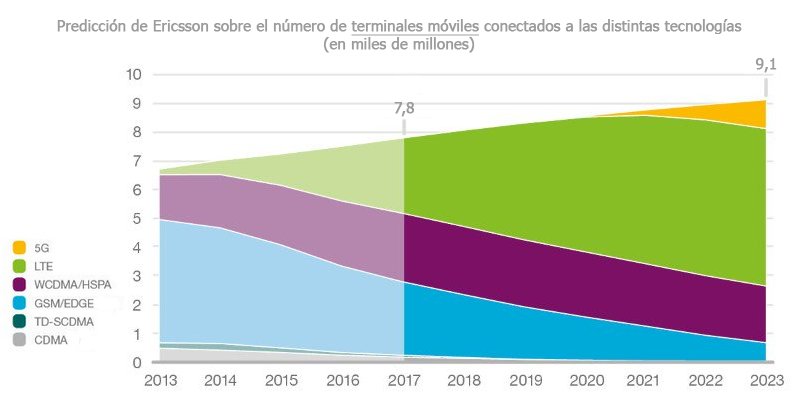
\includegraphics[width=1\linewidth]{imagenes/5gforecast.PNG}
	\caption{Suscripciones móviles por tecnología (en miles de millones) \cite{5gForecastEricsson}}
	\label{fig:5gforecast}
\end{figure}

Con la aparición de las siguientes generaciones, el uso de datos móviles se ha convertido en la finalidad principal de estos dispositivos. Según \cite{informeInicial}, ``El móvil es el dispositivo más utilizado en España para acceder a internet, usado ya por el 94,6 \% de los españoles", asimismo, según la previsión de Cisco \cite{informeInicialCisco}, para el año 2021 existirá un total de 11,6 miles de millones de dispositivos, tanto terminales móviles como otros tipos de dispositivos, conectados a la red móvil en todo el mundo. Esto supondría un tráfico mensual de alrededor de 50 Exabytes a través de la infraestructura de comunicaciones móviles -tres veces más tráfico que en la actualidad-.

\subsection{El futuro de las redes inalámbricas. 5G, \textit{hetnets} y Horizonte 2020}

Con el propósito de hacer frente a las características que las infraestructuras de red han de reunir en el futuro, resultan cruciales las labores de investigación y desarrollo para el establecimiento de nuevos estándares que permitan la coexistencia de dispositivos de distinta naturaleza, ya que las actuales tendencias hacen que empiece a surgir la distinción entre Internet de terminales móviles e Internet de las Cosas, \ac{iot}, siendo de esperar que el número de dispositivos conectados crezca considerablemente año tras año.


Actualmente, es la comunicación de quinta generación, \ac{5g} el estándar que se encuentra en pleno desarrollo y que será el sucesor de la cuarta generación, \ac{4g}. Este estándar pretende ofrecer servicios con una muy alta capacidad, conectividad masiva, muy baja latencia, muy alta seguridad, consumo de energía muy bajo y una calidad de servicio, \ac{qos} extremadamente alta \cite{comparative5G}.

\begin{table}[h]
\centering
\caption{Objetivos de 5G \cite{cognitive5G}.}
\label{tab:5gfeatures}
\resizebox{\textwidth}{!}{%
\begin{tabular}{@{} >{\centering\arraybackslash}m{2.5cm} >{\centering\arraybackslash}m{3.5cm} m{7cm} @{}}
\toprule
\multicolumn{2}{c}{\textbf{Escenario de Aplicación}}    & \multicolumn{1}{c}{\textbf{Requisitos y Desafíos}}                                                                                                         \\ \midrule
\multirow{2}{*}[-17pt]{Internet móvil} & Cobertura extensa & Ofrecer un servicio de alta velocidad, en cualquier momento, en cualquier sitio y en escenarios difíciles como áreas remotas.                              \\ \cmidrule(l){2-3} 
                                & Capacidad masiva      & Ofrecer servicio a usuarios con ratios de transmisión extremadamente altos, y hallar las características que las redes de alto flujo de datos necesitarán. \\ \midrule
\multirow{2}{*}[-30pt]{IoT}            & Conectividad masiva   & Ofrecer capacidad para más de un millón de conexiones simultáneas, y asegurar a los terminales un consumo extremadamente bajo de energía.                  \\ \cmidrule(l){2-3} 
                                & Baja Latencia         & Ofrecer a los usuarios un retardo de menos de 1 milisegundo punto a punto, y cerca de un 100\% de fiabilidad.                                                       \\ \bottomrule
\end{tabular}%
}
\end{table}

En concreto, 5G propone un enfoque disruptivo de las comunicaciones. Debido a la gran cantidad de terminales que estarán conectados simultáneamente y su constante expansión, es primordial ofrecer servicio a todos ellos, tanto en entornos con una densidad de usuarios extremadamente alta como en entornos rurales en los que existe una mayor dispersión de usuarios. Para ello, los operadores pretenden ampliar el rendimiento de sus servicios a través de sistemas multiantena utilizando tecnología \ac{mimo} y mediante técnicas de modulación y multiplexación más eficientes, al mismo tiempo que se aumenta el ancho de banda y se utilizan frecuencias mucho más altas.


\begin{figure}[ht]
	\centering
    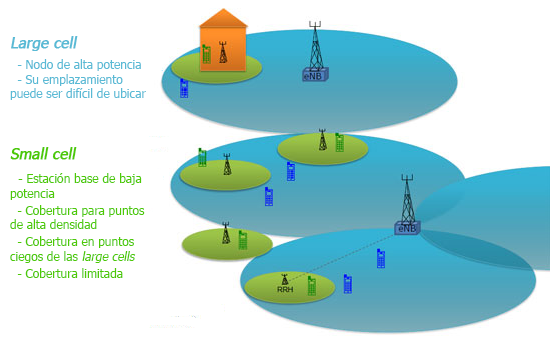
\includegraphics[width=1\linewidth]{imagenes/hetnet_enviroment.png}
	\caption{Entorno típico de \acs{hetnet} \cite{hetnetexplained}}
	\label{fig:hetnet}
\end{figure}

Sin embargo, este conjunto de técnicas y adaptaciones no son suficientes para soportar el uso extremadamente intenso que recibirán las infraestructuras. Por ello, un concepto muy importante en 5G es el de \textit{\acl{hetnet}} (\acs{hetnet}), o lo que es lo mismo, redes heterogéneas en las que conviven nodos o puntos de acceso de diferentes características. En las redes heterogéneas las celdas cuentan con un diferente tamaño según su tipo. De este modo, se distingue entre \textit{macro-, micro-, pico-} y \textit{femto-celdas}. La única diferencia entre ellas a priori es el área de cobertura, la cual es definida mediante la variación de la frecuencia, de la potencia de transmisión y de la altura a la que se encuentra la estación base de la celda en cuestión.


\begin{table}[ht]
\centering
\caption{Características de las clases de celdas.}
\label{tab:celdas}
\begin{tabular}{m{3cm} m{9cm}}
\hline
\multicolumn{1}{c}{\textbf{Tipo de celda}} & \multicolumn{1}{c}{\textbf{Características}}                                                                                                             \\ \hline
Femto-celda                                & Son autónomas y tienen capacidad para apenas unos pocos usuarios. El área que puede cubrir es muy reducida.                                              \\ \hline
Pico-celda                                 & Pueden soportar hasta 100 usuarios simultáneos en áreas de menos de 200 metros. Normalmente se usan en interiores.                                       \\ \hline
Micro-celda                                & De uso urbano, estas celdas pueden cubrir áreas de hasta 1,5 km. En la actualidad, se utilizan para proporcionar cobertura adicional en eventos masivos. \\ \hline
Macro-celda                                & Se puede comparar con las celdas tradicionales. Ofrecen una cobertura máxima de unos 30 km.                                                              \\ \hline
\end{tabular}
\end{table}


A modo de simplificación, se suele utilizar el término \textit{small cell} para hacer referencia a cualquier celda que no sea del tipo \textit{macro-celda}. Se puede comprender un escenario típico de red heterogénea a través de la ilustración de la figura \ref{fig:hetnet}. Como explica dicha figura, en el paradigma de las \acs{hetnet}, las \textit{small cells} se utilizan con triple finalidad: ofrecer cobertura en zonas que las celdas convencionales no cubren, reducir la carga de las macro-celdas y proporcionar servicio en zonas con mayor demanda como interiores o puntos de alta densidad de usuarios (\textit{hot-spots}). Además, 5G pretende incorporar nuevos usos gracias al hecho de disponer de varias estaciones base distintas conviviendo a la misma vez \cite{hetnetexplained}. 

Por ejemplo, una de las posibles mejoras que las redes heterogéneas ofrecen es la de \acl{icic}, ICIC, la cual consiste en la utilización de la interfaz extra con la que cuentan las BS para comunicarse entre ellas con el fin  de reducir interferencias. Para ilustrar el potencial que este conjunto de técnicas ofrece, una de sus implementaciones consiste en delegar el enlace de subida y el enlace de bajada a distintas estaciones base cada uno, de modo que si existe interferencia en uno de los enlaces al nodo conectado, ésta se pueda mitigar utilizando el enlace de menor interferencia para tal uso. Dicha técnica ya ha sido implementada en algunas revisiones de LTE pero gracias a las posibilidades que ofrecen las \textit{small cells}, el rendimiento del enlace podría mejorar notablemente, ya que para 4G solo era posible en casos en los que se recibiera una correcta señal de dos estaciones base a la vez -algo complicado en escenarios con un reuso de frecuencias bajo-, mientras que en redes heterogéneas, son más frecuentes las situaciones cuya calidad de enlace sea aceptable para \textit{small cells} y para \textit{large cells} simultáneamente \cite{ieeeicic}. 

\begin{figure}[!hb]
	\centering
    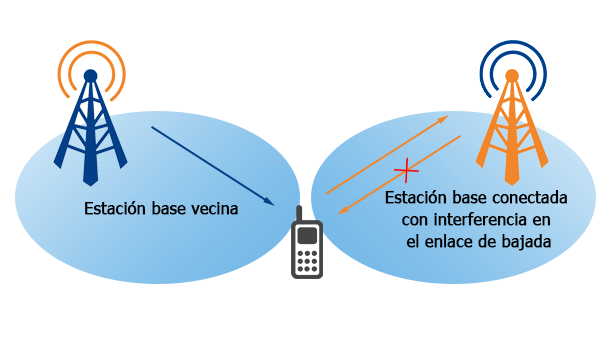
\includegraphics[width=0.75\linewidth]{imagenes/icic.png}
	\caption{Escenario simple en el que se utitiliza una técnica de \acs{icic} para evitar interferencia en el enlace de bajada.}
	\label{fig:icic}
\end{figure}

Como se ha comentado anteriormente y como también se mostraba en el cuadro \ref{tab:5gfeatures}, los retos que se plantean para el desarrollo de 5G no son triviales. Con la finalidad de promover una investigación lo suficientemente eficaz como para abarcar todos los problemas que aparecen sobre la mesa, desde la Administración Pública se han consolidado programas impulsores como el Horizonte 2020 de la Unión Europea, el cual ofrece financiación para proyectos de cualquier naturaleza, incluidos los proyectos de \ac{tic}. Específicamente, el interés en el área \acs{tic} del Horizonte 2020 es conseguir los suficientes avances de consolidación de 5G y de infraestructuras \acs{tic} modernas, sobre todo si explotan el paradigma y/o hacen uso de entornos de IoT, Smart Cities o Big Data, a la vez que se hace hincapié en la ciberseguridad.

Gracias a dicha financiación, pueden ver la luz proyectos como \textit{QuaDRiGa} \cite{quadriga}, un simulador de canal escrito para la plataforma \textit{Matlab} que permite obtener datos realistas de comunicaciones basadas en entornos 5G y \acs{hetnet}. Dicho software será utilizado en este Trabajo de Fin de Grado y, por ello, se dedicará el Capítulo \ref{cap.quadriga} a analizarlo y describirlo con el suficiente detenimiento.

\section{Motivación}

Tal y como se habrá podido deducir de la sección anterior, un reto que suponen las redes heterogéneas es la complejidad de su planificación. El despliegue de numerosas \textit{small cells} junto a las celdas convencionales o nuevas \textit{large cells} agregan un esfuerzo adicional a la hora del diseño de las redes. Es obvia la necesidad de conocer el rendimiento a priori de las redes antes de su desdoble debido a su gran coste y a la suma importancia de ofrecer un servicio óptimo, sin sobredimensionar a la misma vez que se abastece a los usuarios sin sobrecargas.
Además, para un correcto desarrollo de los estándares venideros, como \acs{5g}, es preciso tener en mente los requisitos demandados por el futuro uso de los mismos. No es posible realizar un diseño de un estándar con tanto potencial como 5G sin una reproducción de resultados fiable.

Debido a tal problemática, en etapas de diseño, desarrollo, planificación y despliegue de redes y nuevas tecnologías inalámbricas, los simuladores toman un papel muy importante, puesto que permiten anticiparse a resultados con la finalidad de evitar futuros inconvenientes que un mal diseño pueda provocar, y su consecuente repercusión económica. Del mismo modo, los simuladores también permiten conocer los propios límites de una tecnología y su rendimiento. Algo que aunque solamente tenga un uso inmediato en los campos de investigación, a largo plazo permite evolucionar gracias a revisiones de dichas tecnologías y mejoras en siguientes versiones.

Es por ello que la finalidad del presente Trabajo de Fin de Grado es la elaboración de un simulador de comunicaciones móviles de entornos heterogéneos, con enfoque en \acs{5g}.

\section{Objetivos}

El principal objetivo de este proyecto es utilizar como base el generador de canal de radio \textit{QuaDRiGa} utilizando la plataforma de programación y desarrollo \textit{Matlab} para el desarrollo de un simulador funcional de \acs{5g} que, como elementos fundamentales, incluya terminales móviles y \ac{bs} de tipo micro-celda y macro-celda, a la vez que permita obtener resultados básicos -potencia recibida, interferencias, capacidad de canal...- para distintos criterios de emparejamiento entre estaciones base, y terminales.

Para ello, en primer lugar el alumno debe familiarizarse con el entorno de \textit{QuaDriGa}, teniendo en cuenta que es un simulador de nivel de enlace que está capacitado para su uso a nivel de sistema, así como con el paradigma de comunicaciones móviles, indagando en 5G y en redes heterogéneas especialmente para conocer sus conceptos, metodologías y técnicas.

Seguidamente, es necesario hacer una planificación de las características que el simulador reunirá, descartando las que resulten inviables o aquellas que \textit{QuaDRiGa} no haga posible e implementarlas, modificando el código fuente de \textit{QuaDRiGa} si fuera necesario, y desarrollando sus propios \textit{scripts} y funciones.

El objetivo fundamental de estas etapas es el de extender el simulador de capa física \textit{QuaDRiGa} para obtener un simulador de nivel de enlace más completo con nuevas funcionalidades, incluyendo algunas características propias de simuladores de nivel de sistema, así como también una mayor flexibilidad para evaluar escenarios multi-celda y multi-frecuencia.

Por último, en base al trabajo realizado y al software implementado, se realizarán las oportunas pruebas comprobando el rendimiento de distintos escenarios y ajustes de comunicaciones. También se diseñará un protocolo estándar de pruebas para realizar una comparación exhaustiva.

\section{Organización del Proyecto}

Sección en construcción. Aquí iría un resumen de los siguientes capítulos que será añadido tras la finalización de los mismos.

\paragraph{Capítulo 1: Introducción} \mbox{} \\
	Resumen de la introducción

\paragraph{Capítulo 2: Estado del arte} \mbox{} \\
	Descripción otros simuladores parecidos como New York Sim.

\paragraph{Capítulo 3: Planificación y requisitos} \mbox{} \\
	Requisitos y tareas que hay que realizar para que el proyecto resulte satisfactorio. Diagrama de Gantt.

\paragraph{Capítulo 4: Acerca de \textit{QuaDRiGa}} \mbox{} \\
	Descripción de Quadriga, funcionalidades, limitaciones, explicación de su paradigma, descripción de sus principales funciones, pequeñas pruebas e incluso un breve tutorial.

\paragraph{Capítulo 5: Diseño e implementación} \mbox{} \\
Una explicación detallada de toda la funcionalidad del código del proyecto, cómo se ha logrado, cómo se utiliza...

\paragraph{Capítulo 6: Pruebas} \mbox{} \\
Pruebas y resultados, protocolo de pruebas, consumo de CPU y memoria.

\paragraph{Capítulo 7: Conclusiones} \mbox{} \\
Conclusiones, defectos y puntos fuertes de QuaDRiGa, defectos y puntos fuertes de nuestro simulador, futuros pasos.

%\section{Alcance del trabajo}
%
\chapter{Estado del arte}\label{cap.estado del arte}

\section{Introducción}

Puesto que en el anterior capítulo se hizo especial hincapié en la importancia de los simuladores, este segundo capítulo está dedicado a exponer las principales implementaciones de simuladores orientados a 5G que existen en la actualidad, resaltando las diferencias entre ellas. Por último, se justifican las características que, como objetivo, debe reunir el simulador implementado en el actual proyecto.

Antes de describir los diferentes simuladores existentes a día de hoy, es importante tener en cuenta los tipos de nivel funcional de los simuladores de comunicaciones móviles atendiendo a sus características:
\begin{itemize}
    \item \textbf{Simulador de capa física:} modela las comunicaciones básicas entre un transmisor y receptor teniendo en cuenta parámetros como la posición de los mismos, la frecuencia, el tipo de canal, la trayectoria de la onda y las pérdidas de propagación.
    \item \textbf{Simulador de nivel de enlace:} cuenta con la capacidad de calcular parámetros como la cobertura, potencia o análisis de obstáculos. Además incluye funcionalidades -a veces limitadas- de emparejamiento terminal-estación base y/o control de errores.
    \item \textbf{Simulador de nivel de sistema:} computa parámetros y datos específicos como control de admisión, gestión de carga o eficiencia, incluyendo en ocasiones posibilidad de estudio de uso de ciertos protocolos en la red.
\end{itemize}

A continuación, se enumeran los principales simuladores de 5G desarrollados tanto a nivel de enlace como a nivel de sistema.

\section{NYUSIM Channel Simulator}
\subsection{Introducción}
\ac{nyusim} \cite{nyusim} es un simulador de canal (nivel de enlace) escrito en \textit{Matlab} con el ánimo de generar respuestas al impulso de diversos canales, en dominio espacial y en dominio temporal, con compatibilidad con el modelo de 3GPP pero con ciertas diferencias según sus propios desarrolladores explican en sus publicaciones. Ha sido desarrollado por la Escuela de Ingeniería de la Universidad de Nueva York y está disponible para su libre descarga y distribución en su página web.

Se considera el análogo de \textit{QuaDRiGa} debido a que reúnen características similares y la misma concepción: son simuladores de canal que pretenden modelar comunicaciones móviles de acuerdo a los estándares de 3GPP.
\subsection{Características}
La característica que abandera a este simulador es su capacidad de simular enlaces de radio en frecuencias entre 2 y 73 GHz, un rango bastante extenso que tiene en cuenta las frecuencias de todas las futuras comunicaciones 5G. Sus estaciones base cuentan con la posibilidad de ser modeladas mediante antenas MIMO. Además, considera numerosos tipos de escenario, distinguiendo los casos con y sin visión directa, \ac{los}, junto con pérdidas por penetración de exterior a interior, \ac{o2i}, y el modelado clásico de 3GPP para casos sin visión directa, \ac{nlos}, de descomponer la señal en un total de 20 trayectorias distintas, cada uno con un retardo, una amplitud y un desfase distintos.

\section{WiSE}
\subsection{Introducción}
\ac{wise} \cite{wise} es un simulador de nivel de sistema para redes móviles \acs{lte} y 5G concebido en un principio para su uso exclusivo en simulaciones 4G. Fue desarrollado por investigadores de la \textit{National Central University} de Taiwan y ha sido validado en campañas de calibración del 3GPP.
\subsection{Características}
\acs{wise} integra la capacidad de simular celdas de entornos urbano y rural, tanto micro celdas como macro-celdas así como \textit{Hot-spots} de interiores y alta densidad. Soporta frecuencias de hasta 100 GHz y modelado de canal en 3D. Además, integra posibilidad de movilidad de usuarios, de simular edificios y de grandes anchos de banda.

\section{GTEC}
\subsection{Introducción}
Desarrollado por el Grupo de Tecnología Electrónica y Comunicaciones de la Universidad de A Coruña, GTEC \cite{gtec} se trata de un simulador de nivel de enlace modular que integra la evaluación de entornos de 4G y 5G. Aunque no está basado en simulaciones estándares como los anteriores simuladores, ofrece la posibilidad de ser personalizado y configurado al gusto, gracias a su estructura modular que permite modificar cualquier parámetro fácilmente.
\subsection{Características}
Además de su peculiaridad de ser modular, el simulador GTEC cuenta con capacidad de crear capas de simulación de enlaces que utilizan \ac{ofdm} o bien \ac{fbmc} como forma de onda. Además, cuenta con diferentes modelos de canal obtenidos de resultados experimentales propios y permite realizar medidas al momento en diferentes escenarios.

\section{Vienna}
\subsection{Introducción}
Vienna \cite{vienna} es una \textit{suite} de simuladores escritos en \textit{Matlab} que incluye simuladores de nivel de enlace y de nivel de sistema para \acs{lte} y actualmente, solo un simulador a nivel de enlace para 5G, mientras que el simulador de nivel de sistema se encuentra en desarrollo, todos ellos implementados por investigadores de la Universidad Técnica de Viena. Se distribuye con una licencia de uso exclusivamente académico.
\subsection{Características}
El simulador de nivel de enlace de 5G actualmente incluye características distintivas con respecto a los demás simuladores como la elección de parámetros individualmente para cada nodo, la separación de los canales de subida y de bajada, simulación multi-portadora o diversidad de receptores. Sin embargo, no admite planificación geométrica de la red ni cuenta con un modelo de pérdidas de propagación.

\section{Conclusiones}
Teniendo en cuenta los simuladores anteriormente descritos, se puede extraer como conclusión que es deseable que un simulador de nivel de enlace o de sistema para 5G reúna como características la posibilidad de explotar al máximo las ventajas que 5G ofrece, como pueden ser la posibilidad de simular estaciones base de distinta frecuencia, movilidad de terminales, distintos tipos de celda, planificación geométrica, emparejamiento dinámico, simulaciones a muy altas frecuencias, alta disponibilidad -esto es, contar con un nodo de respaldo al que conectarse-, modelado de distintos tipos de entorno y de canal y modelado de antenas de las estaciones base mediante \acs{mimo}.

Si bien \textit{QuaDRiGa} no incluye todas estas características puesto que se concibe como un generador de canal en el que otros simuladores pueden basarse, como se explica en el Capítulo 4, se puede adelantar del mismo que las funcionalidades que debe incluir un simulador de un nivel superior a \textit{QuaDRiGa} son las de combinar escenarios con distintos tipos de celda, simulaciones multi-frecuencia, modelado de emparejamientos -incluidos los emparejamientos para terminales en movimiento- y obtención de parámetros concluyentes como cálculo de la capacidad del canal (\textit{troughput}) o del \ac{sinr}.
%
\chapter{Planificación y requisitos}\label{cap.requisitos}
\section{Introducción}
Bla bla bla
%
\chapter{Acerca de Quadriga}\label{cap.quadriga}
\section{Introducción}
El corazón de \textit{5Gneralife} está basado en \textit{QuaDRiGa} en su totalidad, por lo que resulta conveniente conocer previamente su funcionamiento y sus nociones básicas antes de detenerse a detallar la implementación del simulador en sí.

\textit{QUAsi Deterministic RadIo channel GenerAtor, QuaDRiGa} es un proyecto cuya finalidad es facilitar el desarrollo de simuladores de redes móviles de nivel de sistema, gracias a su función, que no es otra que generar respuestas impulsivas realistas para distintos canales de radio modelados de acuerdo a diversos estándares. En concreto, en su última versión hasta la fecha (v2.0), \textit{QuaDRiGa} integra un total de 78 modelos de canal, incluidos modelos de acuerdo a estándares creados por diversas entidades como 3GPP o WiNNER \cite{winner} o mmMAGIC.

Aunque \textit{QuaDRiGa} fue concebido para su uso en LTE, las actualizaciones más recientes han hecho compatible su uso con simulaciones orientadas a 5G mediante implementaciones como un rango más amplio de frecuencias, integración de MIMO en las antenas o inclusión de modelos de \textit{small cells} para los distintos entornos.

En este capítulo se especificarán sus principales características y especificaciones, así como su estructura de programación y su modo de uso.

\section{Características}

Puesto que \textit{QuaDRiGa} no pretende ser un simulador independiente, sino un recurso del que se pueden servir otros simuladores como el que ha sido desarrollado, no integra funcionalidades típicas de simuladores como datos característicos del entorno simulado.

Teniendo esto en cuenta, entre sus características generales, podemos destacar:

\begin{itemize}
    \item Permite configuración libre de capas de red con varios transmisores y receptores.
    \item Posibilidad de crear enlaces MIMO.
    \item Su rango de frecuencias es de 450 MHz hasta 100 GHz.
    \item Modela la evolución en el tiempo de sus elementos incluyendo parámetros de pequeña y gran escala.
    \item Modela escenarios rurales y urbanos, interiores y exteriores, todos ellos incluyendo los casos con visión directa (LOS) y sin visión directa (NLOS), con posibilidad de transición entre ellos por parte de los usuarios. Para estos modelos se hace uso de los parámetros establecidos por WINNER+ y por 3GPP-3D.
    \item Implementación completa para Matlab, con programación orientada a objetos. Compatibilidad con algunas versiones de Octave.
\end{itemize}

Una de las características más interesantes y que caracteriza a \textit{QuaDRiGa} es la posibilidad de implantación de distintos tipos de escenario en una misma simulación. Esta funcionalidad pretende modelar el comportamiento de un usuario que se encuentra en movimiento, ya sea a pie o en vehículo, ya que las condiciones de su entorno cambian constantemente a lo largo del recorrido.

\begin{figure}[h!]
	\centering
    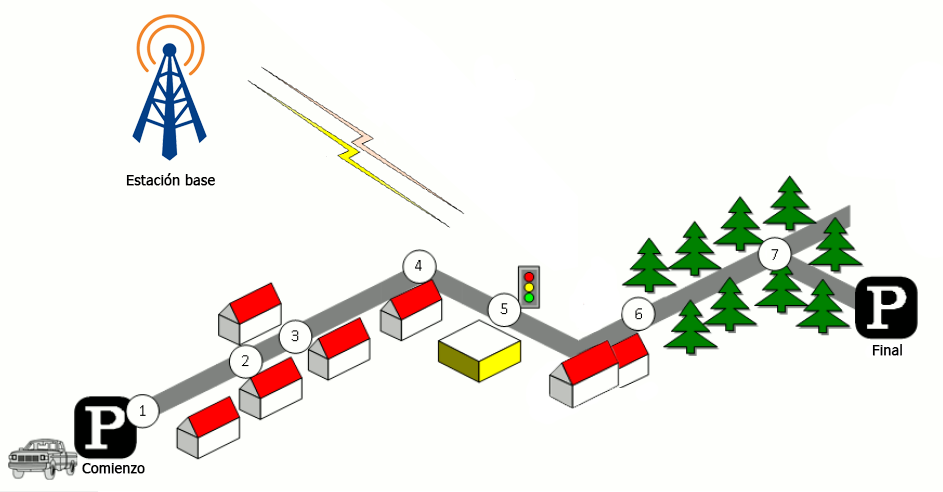
\includegraphics[width=\linewidth]{imagenes/transiciones.png}
	\caption{Ilustración de un entorno de transiciones entre escenarios.}
	\label{fig:transicion}
\end{figure}

Para ejemplificar mejor el concepto de transiciones de la filosofía de implementación de \textit{QuaDRiGa}, se ha realizado una modificación de la figura de su documentación técnica \cite{quadrigadoc} visible en la Figura \ref{fig:transicion}. En ella se puede distinguir un total de seis segmentos cuya transición entre ellos se delimitan con los círculos blancos:

\begin{enumerate}
    \item En (1) se comienza el trayecto y se establece una conexión con la estación base con visión directa LOS en un entorno urbano.
    \item En el punto (2) se cambia de LOS a NLOS.
    \item En (3) se cambia de NLOS a LOS.
    \item Un cambio de dirección sin cambiar las condiciones de recepción (LOS).
    \item Se efectúa una parada con su consecuente cambio de velocidad mientras se mantienen las condiciones de visión directa.
    \item Se produce en (6) un cambio de entorno puesto que se accede a una zona rural. Las condiciones cambian de un escenario urbano con visión directa a uno rural sin visión directa (Urban LOS \(\rightarrow\) Rural NLOS).
    \item Antes de finalizar el trayecto, en (7) se produce un cambio de dirección sin cambiar las condiciones de no tener visión directa.
\end{enumerate}

Como se ha podido observar, este comportamiento típico de usuarios conlleva tener en cuenta varios cambios en las condiciones de recepción por parte del terminal, puesto que se deben considerar parámetros como el tipo de entorno, la visión directa, velocidad y  posición. \textit{QuaDRiGa} hace frente a esta problemática gracias a su modelado de tres dimensiones del entorno junto a la implementación de fusión de parámetros de canal generados, es decir, al generar los coeficientes de canal para un receptor, tiene en cuenta los cambios de tramos para que todos los coeficientes se encuentren correlados entre sí.

Sin embargo, el modelado de transiciones de escenario se encuentra intrínseco en el objeto dedicado al receptor, por lo que su utilidad se ve limitada a estudios de cambios de entorno -por ejemplo, cambio de entorno rural a urbano- pero al no ser un atributo propio de las estaciones base, esta funcionalidad no se puede utilizar para modelar distintos tipos de celda, por tanto, sería una tarea que el simulador de un nivel más alto debe implementar.

Lo que sí resulta útil para un simulador y que puede ser un atributo propio de las estaciones base y los terminales es la transición de LOS a NLOS y viceversa, con en el punto (2) y (3) de la Figura \ref{fig:transicion} puesto que \textit{QuaDRiGa} dispone de recursos que permiten simular la probabilidad de visión directa.

\section{Especificaciones técnicas}

Como se comentó anteriormente, \textit{QuaDRiGa} se sirve de Matlab como plataforma base de desarrollo. Esto ha hecho posible que la última versión hasta la fecha (v2.0.0) esté implementada totalmente con programación orientada a objetos, lo que permite una mayor flexibilidad, rendimiento y sencillez de uso.

Aunque la carga computacional de \textit{QuaDRiGa} puede resultar demasiado pesada según qué escenarios se quieran generar, sus requisitos mínimos de ejecución no resultan muy exigentes tal y como aparece en la Tabla \ref{tab:espec_quadriga}:

\begin{table}[h!]
\centering
\caption{Requisitos mínimos de QuaDRiGa}
\label{tab:espec_quadriga}
\begin{tabular}{c|c}
\textbf{Característica} & \textbf{Requisito mínimo} \\ \hline
Versión de Matlab       & 7.12 (R2011a)             \\
Toolbox                 & Ninguna                   \\
Memoria (RAM)           & 1 GB                      \\
Procesador              & 1 GHz un solo núcleo      \\
Almacenamiento          & 50 MB                     \\
Sistema operativo       & Linux, Windows, Mac OS   
\end{tabular}
\end{table}

Su instalación es sencilla, basta con añadir a Matlab el directorio en el que se encuentran los ficheros descargados con el comando \textit{addpath}:

\begin{lstlisting}[style=Matlab-editor, basicstyle=\tiny]
addpath('/[ruta hasta quadriga]/quadriga_src')
\end{lstlisting}

Una vez instalado, se puede hacer uso de sus funciones para crear entornos de simulación, como se explicará en el siguiente apartado.

\section{Visión de conjunto del software}

Esta sección está dedicada a ilustrar el funcionamiento de \textit{QuaDRiGa} plasmando así los resultados obtenidos de la fase de aprendizaje y toma de contacto con el generador. En primer lugar se detallarán sus pautas de uso, aclarando su estructura interna y el enfoque desde el que se debe usar. Seguidamente, se realizará una prueba para demostrar sus capacidades y plantear sus limitaciones, que serán la antesala y la motivación para el siguiente capítulo dedicado a la íntegra implementación del simulador.

\subsection{Estructura del software y utilización}

En primer lugar, es conveniente tener en consideración la estructura de software con la que cuenta \textit{QuaDRiGa}. Este generador implementa un total de siete clases para su procesamiento, cuatro de ellas implementan parámetros de entrada, dos están dedicadas a cómputos internos, y una última clase que engloban los resultados de salida.

De las clases que se utilizan como entrada podemos diferenciar:
\begin{itemize}
    \item \textbf{\textit{qd\_simulation\_parameters}} define ajustes generales como frecuencias y densidad de muestreo.
    \item \textit{\textbf{qd\_arrayant}} esta clase sirve para modelar las antenas que las estaciones base y los terminales móviles integran en sus comunicaciones, incluida la opción del modelaje MIMO.
    \item \textbf{\textit{qd\_track}} genera los objetos de seguimiento de terminales móviles. Sirve para modelar principalmente el movimiento de los usuarios y sus transiciones de escenario.
    \item \textbf{\textit{qd\_layout}} combina los seguimientos de receptores y los parámetros de simulación para generar capas de simulación independientes, una por cada frecuencia o tipo de estación base. Modela las posiciones de las estaciones base.
\end{itemize}

Por otro lado, en cuanto a las clases de procesamiento interno:

\begin{itemize}
    \item \textbf{\textit{qd\_sos}} se encarga de generar señales correladas entre sí basándose en el método conocido como \textit{suma de sinusoides}. Esta señales se utilizan para obtener parámetros sobre la señal recibida por parte de las estaciones móviles. 
    \item \textbf{\textit{qd\_builder}} crea los coeficientes de canal generando parámetros de gran escala y canales independientes para cada una de las antenas en el caso de usar modelado MIMO para las mismas.
\end{itemize}

Por último, la salida se modela con una séptima clase que engloba el resultado final derivado del uso del resto de las clases:

\begin{itemize}
    \item \textbf{\textit{qd\_channel}} contienen los datos de coeficientes de canal que se obtienen como resultado de las anteriores configuraciones. Esto incluye parámetros como amplitud y retardos de cada uno de las trayectorias del modelo de canal utilizado por \textit{QuaDRiGa}. También se encarga de fusionar las secuencias de muestras temporales del entorno para realizar una evolución temporal continua y coherente del escenario de simulación.
\end{itemize}

Cada una de las clases implementan atributos y métodos propios que por lo general sirven para generar a su vez objetos de otras clases o parámetros de salida. Además, todas las clases están perfectamente relacionadas entre sí, por lo que el mejor método para describir relaciones entre clases y los nombres de sus atributos y/o métodos es el uso de un diagrama como el de la Figura \ref{fig:uml_quadriga}, extraído de su propia documentación técnica \cite{quadrigadoc}.

% Diagrama UML

\begin{figure}[ht!]
	\centering
    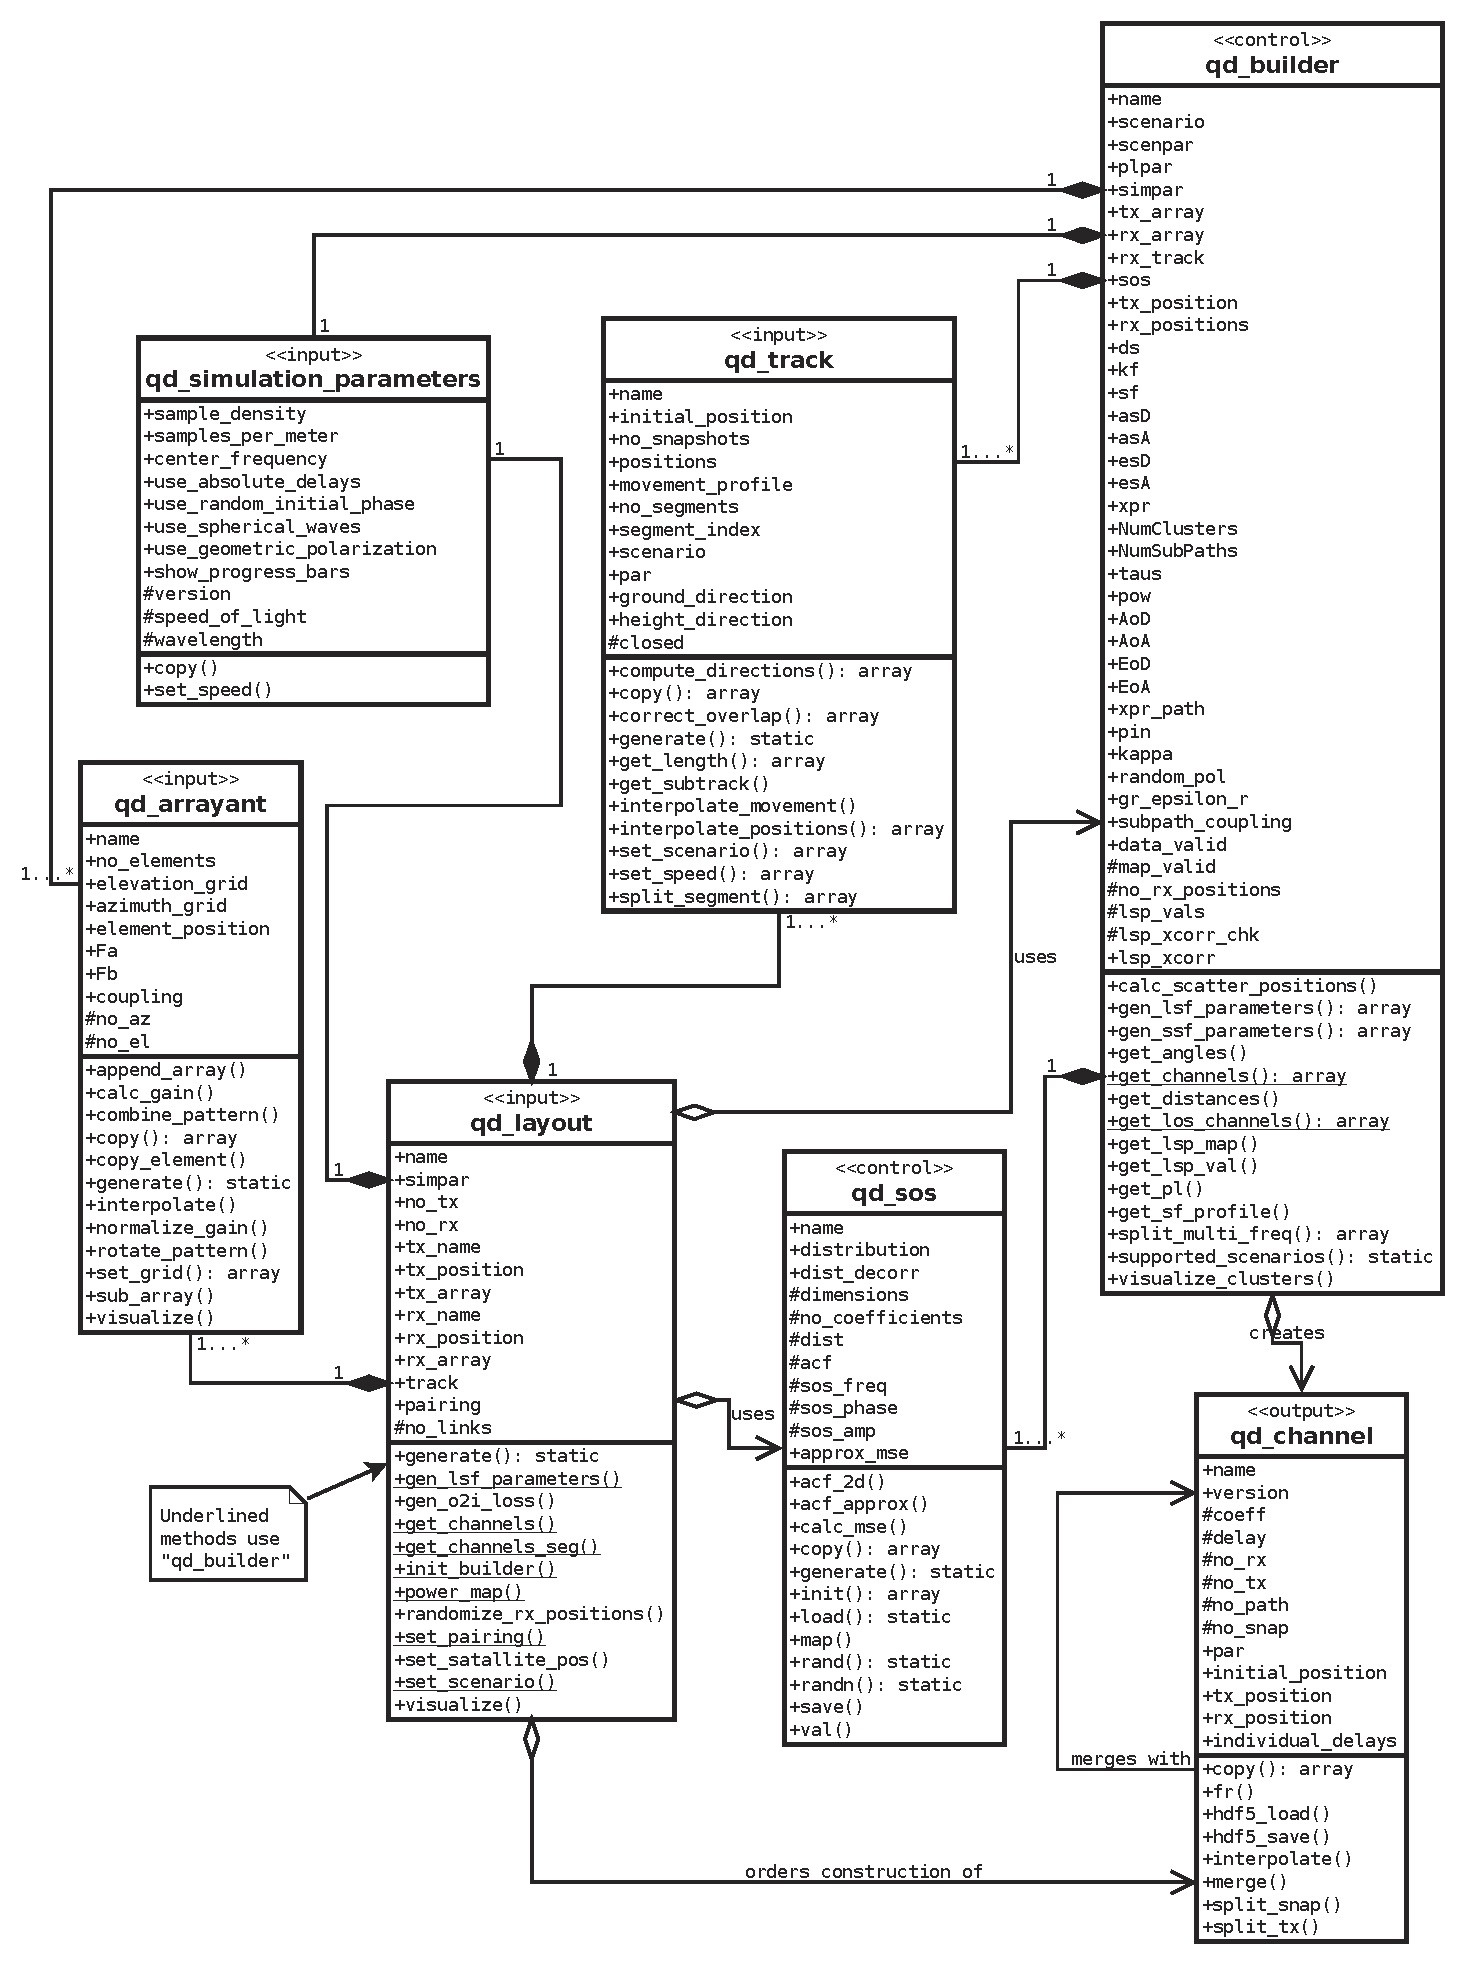
\includegraphics[width=\linewidth]{imagenes/uml_quadriga.png}
	\caption{Diagrama de clases UML de QuaDRiGa.}
	\label{fig:uml_quadriga}
\end{figure}

% Pasos de uso

Cada simulación en \textit{QuaDRiGa} está hecha en tres pasos más un cuarto paso opcional, obteniendo como resultado un objeto de la clase \textit{qd\_channel}:

\begin{enumerate}
    \item Configurar escenario. Esto conlleva la declaración de objetos de las cuatro clases que se toman como entrada, los cuales modelan antenas -tanto para receptor como emisor, para lo cual \textit{QuaDRiGa} ya incluye sus propios modelos predeterminados-, seguimiento de terminales móviles -especificando patrón de movimiento, distancia recorrida, etc.-, escenarios para terminales y/o estaciones base y, por último, capas de simulación que, como se mencionó anteriormente, están caracterizados por parámetros como frecuencia de trabajo, posiciones de estaciones base o emparejamientos entre estaciones base y terminales.
    \item Generar parámetros de gran escala correlados. Esto se hace mediante el uso de la clase \textit{qd\_sos} que a través de los parámetros extraídos de la base de datos de canales que integra \textit{QuaDRiGa}, genera señales aleatorias a través del método de suma de sinusoides.
    \item Calcular los coeficientes de canal fusionados y correlados a través de la clase \textit{qd\_builder} que unifica todos los objetos de entrada más las señales generadas en el paso número 2 para obtener coeficientes de canal representados mediante sus amplitudes, desfases y otros parámetros como ángulos de llegada. Además, se ofrece la opción de obtener dichos coeficientes en dominio de la frecuencia para posibles procesados posteriores.
    \item Post-procesado (opcional). Dentro de los procesados posteriores, más allá del método que implementa la clase dedicada a los canales, no existen más herramientas que permitan obtener resultados más representativos o concluyentes sobre la simulación. Por ello, en este cuarto paso es donde se centra la labor de desarrollo del simulador, como se verá en el Capítulo \ref{cap.implementacion}.
\end{enumerate}

\subsection{Capacidades y limitaciones. Demostración práctica}

Una vez que se adquiere una visión general sobre \textit{QuaDRiGa}, su uso y los conceptos que engloba, es posible realizar un uso estándar del mismo. En esta sub-sección se realizará un ejemplo de simulación utilizando únicamente \textit{QuaDRiGa} con la finalidad de plasmar sus funcionalidades y sus carencias, de modo que podrá ser comparado con futuros ejemplos de uso de \textit{5Gneralife}.

En primer lugar, señalar su uso exclusivo mediante línea de comandos y/o \textit{scripts}, lo cual puede resultar abstracto para un usuario que comience a usar \textit{QuaDRiGa}, especialmente en casos en los que dicho usuario nunca antes haya realizado una toma de contacto con un simulador de comunicaciones móviles.

Como solamente se puede controlar por línea de texto, para este ejemplo se ha desarrollado un \textit{script} que pretende simular una capa de simulación para un entorno de macro-celdas completamente urbano. Dicha capa contará con 10 receptores en movimiento, recorriendo cada uno 1 km. Además, se incluirá un total de tres estaciones base. Tanto terminales como estaciones base tendrán una posición aleatoria y sus antenas serán omnidireccionales de ganancia 5 dBi para simplificaciones. La frecuencia de trabajo será de 2,6 GHz.

Para la puesta en marcha del escenario, el primer paso es la configuración de parámetros de simulación, tarea que solamente precisa de crear un objeto de la clase \textit{qd\_simulation\_parameters} y modificar su atributo de frecuencia a 2,6 GHz:

\begin{lstlisting}[style=Matlab-editor, basicstyle=\tiny]
%% Parametros de simulacion
sim_param = qd_simulation_parameters; % Se genera un objeto de parametros
sim_param.center_frequency = 2.6e9;   % Frecuencia de 2,6 GHz
\end{lstlisting}

A continuación, se hace el proceso análogo para crear dos objetos de la clase \textit{qd\_arrayant} que modelarán sendas antenas omnidireccionales, una para cada tipo de elemento de la simulación -terminales y estaciones base-:

\begin{lstlisting}[style=Matlab-editor, basicstyle=\tiny]
%% Antenas
antenaMT = qd_arrayant('omni'); % Asignacion de antena omnidireccional de ganancia 5 dBi
antenaBS = qd_arrayant ('omni');
\end{lstlisting}

Acto seguido, se realiza la elaboración de la capa de simulación. Como en este caso no existe más de un tipo de celda ni más de una frecuencia, solo es necesario crear una capa. La capa integra los datos sobre estaciones base y receptores, así como el tipo de entorno. En primer lugar se crea el objeto y se configuran los emisores y receptores con el número de cada uno de ellos y sus corresponientes antenas:

\begin{lstlisting}[style=Matlab-editor, basicstyle=\tiny]
%% Transmisores y receptores

layout_uma = qd_layout(sim_param); % Generamos capa de simulacion
layout_uma.no_tx = 3; % 3 estaciones base
layout_uma.no_rx = 10; % 10 usuarios

layout_uma.rx_array = antenaMT; % Asignacion de antena de terminal
layout_uma.tx_array = antenaBS; % Asignacion de antena de BS
\end{lstlisting}

Acto seguido, se configuran las posiciones de los mismos. Para ello se hace uso del método \textit{randomize\_rx\_positions} para los receptores, y un pequeño bucle \textit{for} para los transmisores. Se ha decidido que la distancia máxima del centro a la que pueden estar los elementos sea de 2 km:

\begin{lstlisting}[style=Matlab-editor, basicstyle=\tiny]
%% Posiciones
% Posiciones de usuarios aleatorias con altura de 1,5 m:
layout_uma.randomize_rx_positions(2000, 1.5, 1.5, 0); 

% Posiciones de Bs aleatorias:
for i = 1:layout_uma.no_tx
    pos_x = randi(4000) - 2000; % Posicion X aleatoria entre -2000 y 2000 m del centro
    pos_y = randi(4000) - 2000; % Posicion Y aleatoria entre -2000 y 2000 m del centro
    altura = 25; % 25 metros de altura
    layout_uma.tx_position(:, i) = [pos_x, pos_y, altura];
end
\end{lstlisting}

Para completar la configuración de la capa, es necesario modelar los dos últimos aspectos del escenario: el entorno y el movimiento de los usuarios. Para el movimiento, se ha utilizado un modelado de calle que \textit{QuaDRiGa} implementa, con una orientación aleatoria entre 0 y 360 grados, una longitud mínima de 50 m para las calles, una media de longitud de calle de 187 m, una desviación típica de 83 metros para su longitud, un radio de curva de 10 metros para los giros y una probabilidad de girar en un cruce de 0,5 -según la documentación de \textit{QuaDRiGa} es la son los datos obtenidos para modelar las calles de Berlín-. Para el tipo de entorno, se utiliza el método \textit{set\_scenario} tanto para el objeto de \textit{layout} como para cada uno de los objetos \textit{track}, especificando un tipo de entorno de acuerdo al estándar de macro-celda urbana especificado por 3GPP-3D \cite{3gpp3d}, con una probabilidad de visión directa de 0,2, extraído del mismo:

\begin{lstlisting}[style=Matlab-editor, basicstyle=\tiny]
%% Modelado del escenario
NLOS_prob = 0.8; % Probabilidad de NLOS de 80%
layout_uma.set_scenario('3GPP_3D_UMa',[],[]); % Asignacion de macro-celda segun 3GPP-3D

% Generamos movimientos para los usuarios con modelado de calle de Berlin
trk = cell(1);
for a = 1 : layout_uma.no_rx
    trk{1} = qd_track('street', 1000, randi(360), 50, 187, 83, 10, 0.5); % Calle
    trk{1}.initial_position = layout_uma.rx_position(:,a); % Posicion de acuerdo a la inicial
    trk{1}.name = layout_uma.rx_name{a}; % Se asigna un nombre unico
    escenarios = {'3GPP_3D_UMa_LOS', '3GPP_3D_UMa_NLOS'}; % Se asignan escenarios
    trk{1}.set_scenario( escenarios, [1-NLOS_prob, NLOS_prob], [] ); % Se crean segmentos
    layout_uma.track(1,a) = trk{1}.copy; % Se asigna a la capa
end

\end{lstlisting}

Para obtener las variables de salida, el único paso que queda es el de crear un objeto de la clase \textit{qd\_builder} con la finalidad de generar efectos de pequeña escala y finalmente, generar los coeficientes de canal y unirlos para que entre ellos exista correlación. Cabe destacar que el hecho de generar los efectos de pequeña escala aumenta considerablemente el tiempo de ejecución pero permite tener una simulación sustancialmente más realista.

\begin{lstlisting}[style=Matlab-editor, basicstyle=\tiny]
%% Generamos canales
builder = layout_uma.init_builder; % Objeto builder para pequena escala
gen_ssf_parameters( builder ); % Generamos efectos de pequena escala
canales = get_channels( builder ); % Generamos coeficientes de canal
canales_finales = merge( canales );
\end{lstlisting}

Por último, se puede visualizar la capa a través del método que \textit{QuaDRiGa} ofrece, obteniendo como resultado una representación como la de la Figura \ref{fig:repres_ejemplo}.

\begin{lstlisting}[style=Matlab-editor, basicstyle=\tiny]
%% Visualizacion
layout_uma.visualize([],[],2);
\end{lstlisting}

\begin{figure}[h!]
	\centering
    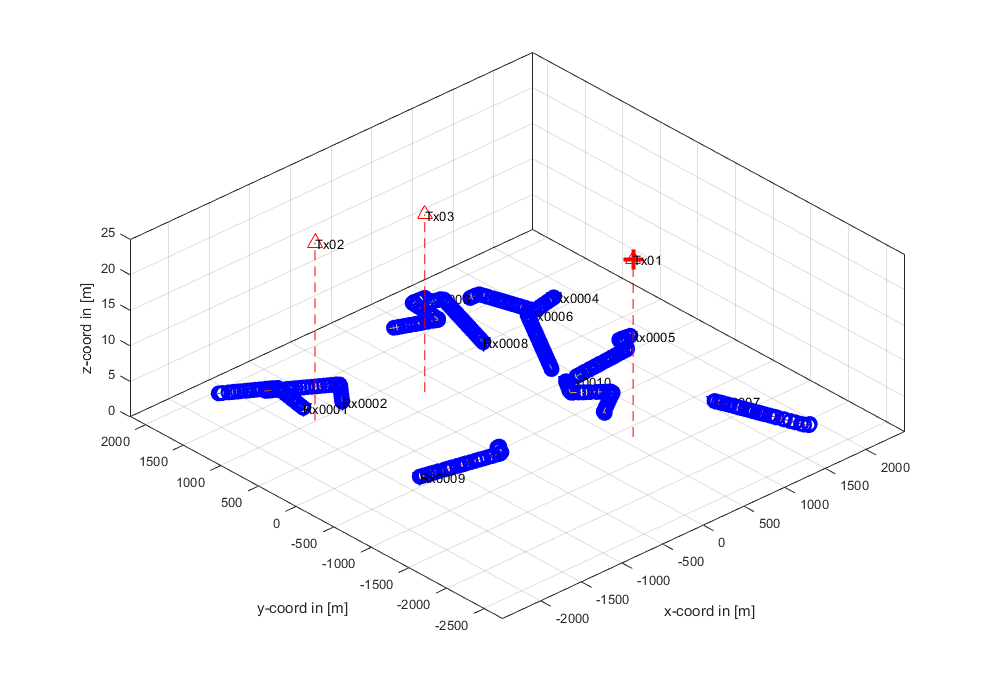
\includegraphics[width=\linewidth]{imagenes/visualizacion_ejemplo.png}
	\caption{Visualización del entorno simulado proporcionada por \textit{QuaDRiGa}.}
	\label{fig:repres_ejemplo}
\end{figure}

Como se observa en la Figura \ref{fig:repres_ejemplo}, se trata de una representación en tres dimensiones que resulta bastante simple a la vez que no detalla ciertos aspectos. Las líneas rojas representan las estaciones base mientras que el cúmulo de puntos es el modo que tiene \textit{QuaDRiGa} de mostrar las trayectorias de sus receptores en movimiento. Si ampliamos la zona de uno de los receptores, se puede diferenciar la línea del recorrido mientras que cada uno de los círculos azules representa un cambio de segmento. En cada transición de segmento se asigna un escenario aleatorio con probabilidad 0.2 para LOS y 0.8 para NLOS. Véase la Figura \ref{fig:receptor_ejemplo}.

\begin{figure}[h!]
	\centering
    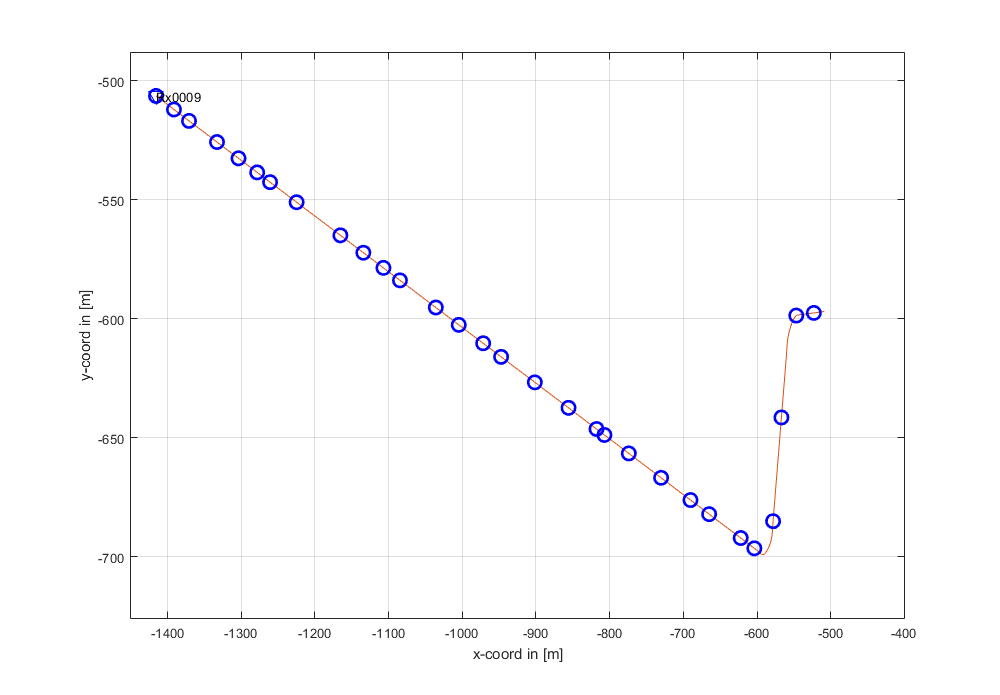
\includegraphics[width=\linewidth]{imagenes/visualizacion_ejemplo_rx1.png}
	\caption{Visualización del recorrido de uno de los receptores.}
	\label{fig:receptor_ejemplo}
\end{figure}

Además, resulta interesante efectuar una indagación en el objeto de la clase \textit{qd\_channel} que se ha generado como salida. Para empezar, la variable \textit{canales\_finales} es un \textit{array} de celdas que cuenta con unas dimensiones de 1x30. Existe un objeto de tipo canal para cada uno de los posibles enlaces, esto es, para cada uno de los 10 receptores, existen 3 objetos de canal, uno `por cada estación base.

Si se abren los datos de uno de los 30 canales, se puede observar la composición del mismo, como muestra la Figura \ref{fig:variable_canal}:

\begin{figure}[h!]
	\centering
    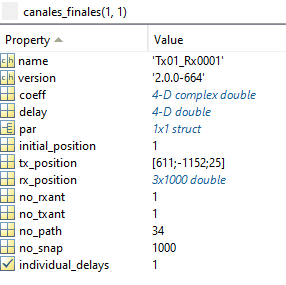
\includegraphics{imagenes/canal_generado_ejemplo.PNG}
	\caption{Estructura de un objeto de la clase \textit{qd\_channel} generado en el ejemplo.}
	\label{fig:variable_canal}
\end{figure}

En primer lugar, se aprecia el nombre del canal que hace referencia a los dos elementos que constituyen el enlace, el transmisor número 1 -Tx01- y el receptor número 1 -Rx01-. Entre los atributos de interés se encuentran las variables \textit{coeff} y \textit{delay}, dos matrices de dimensiones 1x1x34x1000 -dimensiones correspondientes al número de receptores, el número de emisores, el número de trayectorias que el rayo de la señal ha tomado, y el número de posiciones del receptor a través de su recorrido- que contienen las amplitudes y las fases de los coeficientes de canal generados, normalizados. Estos datos a priori no proporcionan información tangible para simulaciones, por lo que es tarea de un simulador basado en \textit{QuaDRiGa} la de procesar posteriormente estos canales con la finalidad de extraer información y obtener datos de caracterización específicos, como podría ser la capacidad del canal.

Como dato a tener en cuenta, el proceso de la simulación de este ejemplo tomó un tiempo de ejecución de 209,25 segundos -3 minutos y medio aproximadamente- utilizando un ordenador de las características que aparecían en la Tabla \ref{tab:caracteristicas}, por lo que es de esperar que para simulaciones más complejas, sean necesarias unas capacidades computacionales considerables.

Para concluir y a modo de resumen, mencionar que para ilustrar el funcionamiento de \textit{QuaDRiGa} con un ejemplo, se ha configurado una entrada compuesta por la generación de objetos que han parametrizado los detalles de la simulación -como por ejemplo la frecuencia de trabajo-. También la capa de simulación incluyendo en ella el número de terminales y su movimiento, el número de estaciones base y su posición, así como el entorno de simulación -en concreto, se ha optado por el modelo 3D de 3GPP publicado en el informe técnico 36.873-. Por otro lado, como salida se ha obtenido un objeto de la clase \textit{qd\_channel}, cuya arquitectura permite obtener las amplitudes normalizadas y las fases de la señal de enlace entre cada uno de los terminales y las estaciones base. También se ha podido obtener una representación visual de la capa de simulación (Figura \ref{fig:esquema_ejemplo}).

% Figura de un esquema
\begin{figure}[ht!]
	\centering
    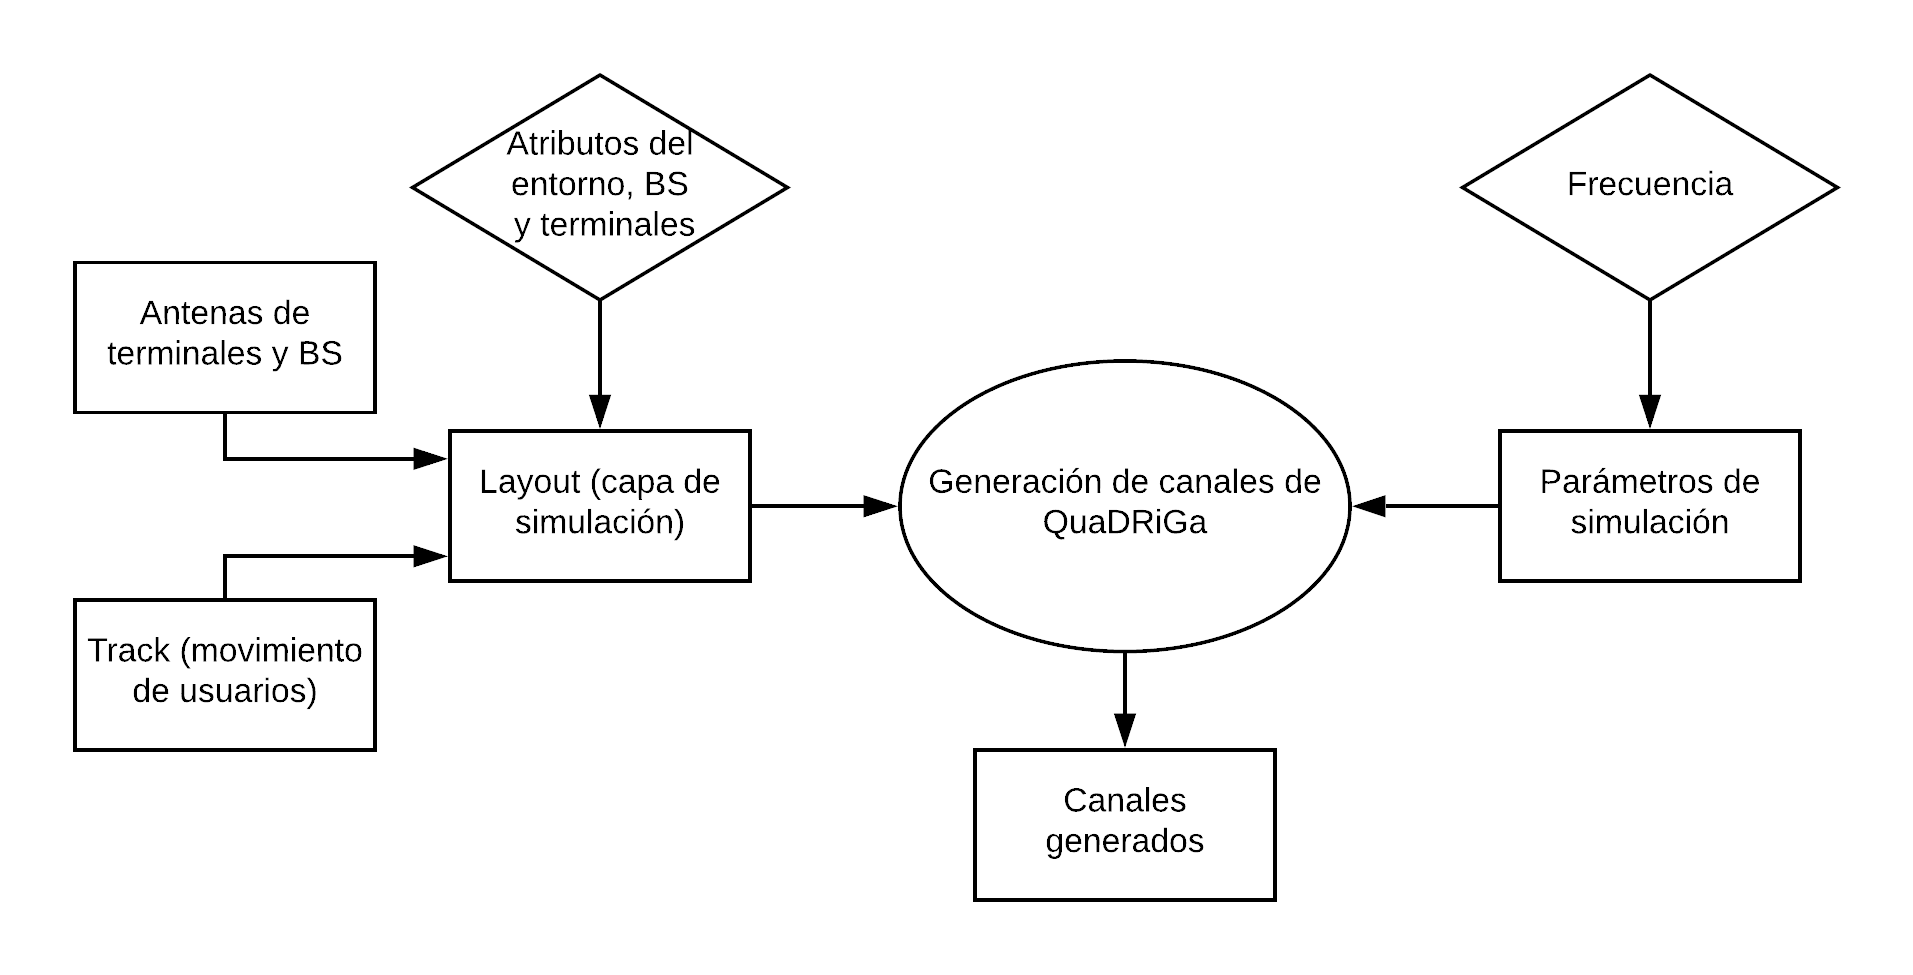
\includegraphics[width=\linewidth]{imagenes/diagrama_ejemplo.png}
	\caption{Diagrama de utilización de \textit{QuaDRiGa}.}
	\label{fig:esquema_ejemplo}
\end{figure}

Si bien estos parámetros de salida son los más dificultosos de obtener debido a su complejidad de cómputo y a la estricta normativa de estándares por los que se rige, no son suficientes y necesitan un procesado extenso para la obtención de datos propios de un simulador. Por ello, el reto que se plantea para implementar un simulador a partir de \textit{QuaDRiGa} como el que se ha desarrollado para este Trabajo de Fin de Grado es el de un código que, de por sí solo, sea capaz de generar e interpretar coeficientes de canal que surjan a partir de configuraciones específicas de 5G, incluyendo, entre otras, funcionalidades de creación de celdas de distinta naturaleza, compartir los mismos usuarios entre todas las capas de simulación -algo que no es posible con \textit{QuaDRiGa}-, obtención de visualizaciones mejoradas y cálculo de parámetros característicos de salida que permitan evaluar objetiva y fácilmente la red creada.


%
\chapter{Diseño e implementación}\label{cap.implementacion}
\section{Introducción}

Este capítulo está dedicado a la profundización en la constitución del propio simulador así como sus funcionalidades, diseño, modo de uso y estructura. La finalidad del mismo es la de plasmar una visión que englobe todos los aspectos característicos del simulador, desde su concepción y desarrollo hasta su alcance y utilidad.

\section{Visión general del simulador}

Este simulador ha sido desarrollado en su totalidad con la plataforma de desarrollo Matlab, implementando y utilizando exclusivamente \textit{scripts}, funciones, objetos y \textit{frameworks} de dicha plataforma.

Este software ha sido concebido como código libre, por lo que está disponible para su consulta, uso y modificación para todo el mundo a través de la plataforma GitHub, protegido bajo una licencia GNU v3.0, al igual que se encuentra \textit{QuaDRiGa}.

Remarcar también que se ha apostado por una estructura que no modifique en nada el código original de \textit{QuaDRiGa}, por lo que se trata de una implementación totalmente independiente, lo que ofrece como principal ventaja la escalabilidad del mismo y la compatibilidad entre ambos programas en futuras actualizaciones.

La filosofía de diseño del simulador ha sido la de ofrecer al usuario un método accesible e intuitivo de acceder a las simulaciones de \textit{QuaDRiGa} permitiendo flexibilidad en las opciones de entrada, así como un post-procesado de las salidas del generador de canal que permitan al usuario entender qué es lo que está sucediendo en su simulación y el comportamiento de la misma. De este modo, se pretende ahorrar el periodo de documentación sobre la utilización de \textit{QuaDRiGa}, que para adquirir unas nociones de uso avanzado se han dedicado 100 horas en el trascurso de este proyecto, como se señalaba en al Tabla \ref{tab:horas}.

Por ello, este simulador es completamente utilizable sin línea de comandos como sucede en la mayoría de simuladores y software escritos en Matlab. Sin embargo, para extraer datos avanzados de la simulación, como valores numéricos de los distintos parámetros que se obtienen de salida, sí que es necesario trabajar en línea de comandos una vez completa la simulación, puesto que el desarrollo del simulador se ha centrado en su valoración visual a través de herramientas como gráficas.

En primer lugar, se comenzará por detallar los requisitos de sistema que se precisan para su ejecución, como muestra la siguiente sub-sección. Acto seguido, se procederá a mostrar sus características de una forma cualitativa, seguido de una lista de mejoras con respecto al software original -\textit{QuaDRiGa}- y, por último, una descripción de su modo de uso y su correcto funcionamiento.

\subsection{Requisitos de ejecución}

Aunque este software no ha sido probado en una amplia variedad de equipos de distintas plataformas, gracias a Matlab, se puede asegurar una compatibilidad fiable en la mayoría de equipos que sean capaces de ejecutar dicha plataforma de desarrollo.

Sin embargo, la capacidad de cómputo que exigen ciertos cálculos que se llevan a cabo durante las simulaciones de \textit{QuaDRiGa}, así como funcionalidades adicionales que se han implementado posteriormente, hacen que los requisitos para ejecutar el simulador resulten más restrictivos que los originales de \textit{QuaDRiGa}. En concreto, en la Tabla \ref{tab:espec_simulador} se puede encontrar los requisitos que se han estimado tras una fase de prueba en el que se ha medido el rendimiento y los recursos que el simulador ha necesitado durante su ejecución:

\begin{table}[h!]
\centering
\caption{Requisitos mínimos del simulador para una compatibilidad total}
\label{tab:espec_simulador}
\begin{tabular}{c|c}
\textbf{Característica} & \textbf{Requisito mínimo} \\ \hline
Versión de Matlab       & R2017a             \\
Toolbox                 & App Designer                   \\
Memoria (RAM)           & 1,5 GB                      \\
Procesador              & 1 GHz un solo núcleo      \\
Almacenamiento          & 80 MB                     \\
Sistema operativo       & Windows, Mac OS   
\end{tabular}
\end{table}

Como se puede observar, si se compara con las especificaciones de \textit{QuaDRiGa} que aparecían en la Tabla \ref{tab:espec_quadriga}, los requisitos han cambiado volviéndose algo más exigentes. Este cambio está justificado debido al Framework utilizado para implementar la interfaz gráfica, \textit{App Designer}, que viene incluido solamente en versiones de Matlab R2017a y superiores. Del mismo se hablará en futuras secciones.

Además, cierto intercambio de instancias entre clases y funciones se realiza a través del almacenamiento de disco duro, por lo que se requiere de un mínimo mayor de capacidad de almacenamiento con la finalidad de permitir esta transacción de datos. 

Puesto que el simulador no es compatible con Octave, se ha perdido la compatibilidad con Linux.

Por otro lado, cabe destacar que estos son los requisitos para una compatibilidad máxima, especialmente con la interfaz gráfica. Sin embargo, es posible ejecutar una versión minimalista disponible en GitHub que solamente requiere la inserción manual de los parámetros de entrada a partir de la creación de variables a través de \textit{script} o línea de comandos. Para esta versión, los requisitos son los mostrados en la Tabla \ref{tab:espec_simulador_minimalista}:

\begin{table}[h!]
\centering
\caption{Requisitos mínimos del simulador para su versión minimalista sin GUI}
\label{tab:espec_simulador_minimalista}
\begin{tabular}{c|c}
\textbf{Característica} & \textbf{Requisito mínimo} \\ \hline
Versión de Matlab       & R2011a             \\
Toolbox                 & Ninguno                  \\
Memoria (RAM)           & 2 GB disponibles                     \\
Procesador              & 1 GHz un solo núcleo      \\
Almacenamiento          & 80 MB                     \\
Sistema operativo       & Windows, Mac OS   
\end{tabular}
\end{table}

Básicamente, los requisitos de esta versión son los mismos que los de \textit{QuaDRiGa} con la salvedad de la necesidad de un mayor espacio de almacenamiento justificado anteriormente, un incremento de memoria RAM debido a la gran cantidad de datos que se almacenarán en la memoria y la pérdida de la compatibilidad con Octave debido a que el desarrollo ha sido exclusivo para Matlab sin tener en cuenta ninguna otra plataforma de desarrollo o de ejecución.

\subsection{Características}

Aunque el simulador esté basado en \textit{QUaDRiGa} para la generación de sus coeficientes de canal, las características con respecto a su base cambian sustancialmente, ya sea por funcionalidades descartadas en el desarrollo, o bien, por nuevas implementaciones añadidas:

\begin{itemize}
    \item Permite la creación de dos tipos de capas de red, una para macro-celdas y otra para micro-celdas, con hasta 37 estaciones base cada una y sin límite de receptores.
    \item Las características de modelado del entorno vienen establecidas de acuerdo a la normativa de 3GPP TR 38.901, que incluye simulaciones con frecuencias en un rango entre 500 MHz y 100 GHz, con una reutilización unitaria.
    \item Diferenciación de segmentos de visión directa y sin visión directa. La probabilidad de los mismos está determinada por el usuario.
    \item Los terminales móviles se encuentran en movimiento. Cuentan con interfaz dual, una a la frecuencia de las macro-celdas y otra a la de las micro-celdas. Ambas capas de simulación son capaces de compartir los mismos usuarios.
    \item La cobertura de las celdas se encuentran modeladas por una antena omnidireccional en el centro de las mismas a modo de simplificación.
    \item Planificación geométrica de las capas de simulación. Una vez establecido el número de celdas, éstas se distribuyen homogéneamente a través de todo el escenario según la distancia de separación entre ellas que se especifique.
    \item Integra evolución de la señal teniendo en cuenta efectos de pequeña y de gran escala.
    \item Por simplificación de implementación y de costes computacionales, los enlaces son de tipo SISO.
    \item Interfaz gráfica de usuario que permite insertar los parámetros de simulación de una forma fácil y cómoda, así como visualizar los resultados y compararlos entre todos ellos.
    \item Dos criterios de emparejamiento: celda más cercana y celda con mayor SINR recibida.
    \item Visualización del escenario mejorada con división de fronteras entre celdas y diferenciación de macro-celdas y micro-celdas, incluyendo leyenda de elementos -Figura \ref{fig:muestra_visualizacion}-.
    \item Incorporación de potencias de transmisión, ruido térmico y asignación de ancho de banda.
    \item Implementación modular y escalable, posibilidad de trabajar con línea de comandos, y de extraer y almacenar parámetros generados.
\end{itemize}

\begin{figure}[h!]
	\centering
    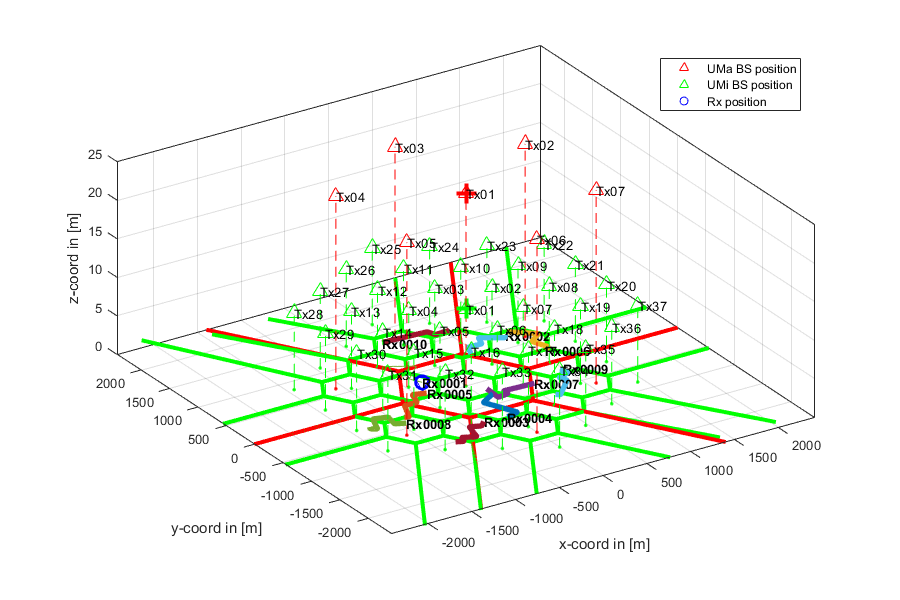
\includegraphics[width=\linewidth]{imagenes/muestra_visualizacion.png}
	\caption{Muestra de la visualización mejorada que implementa el simulador.}
	\label{fig:muestra_visualizacion}
\end{figure}

Gracias a todas estas implementaciones y funcionalidades, \textit{5Gneralife} es capaz de generar un entorno típico de 5G donde conviven celdas de distintos tipos, a altas frecuencias y altos anchos de banda, lo que permite evaluar el comportamiento de una red heterogénea realista con detalles lo suficientemente precisos como para que su comportamiento sea similar a una implementación del mismo tipo. 

\subsection{Lista de mejoras}

Para llegar al simulador se ha elaborado un conjunto de mejoras de \textit{QuaDRiGa} que, implementadas en su conjunto, resultan en \textit{5Gneralife}. Esto implica la elaboración de una nueva clase y de más de una decena de funciones que serán expuestas en la sub-sección de estructura y posteriormente, explicadas con detalle en la sección dedicada a la implementación.

A grandes rasgos, todas estas mejoras se pueden resumir en en el siguiente listado:

\begin{itemize}
    \item \textbf{Mejora 1:} Recopilación de variables de entrada intuitiva y de forma gráfica. Ampliación de parámetros de simulación como ruido o ancho de banda.
    \item \textbf{Mejora 2:} Combinación de celdas de modo que ahora los usuarios en ambas capas de simulación son los mismos. En este simulador, las capas no son independientes. Esto implica que se consigue una implementación de receptores con interfaz dual, una para cada banda de radio, y que no es necesario crear una capa de simulación para cada celda.
    \item \textbf{Mejora 3:} Inclusión de modelado de potencia de transmisión. Los coeficientes de canal que el generador calculaba se encontraban normalizados y no tenían en cuenta potencias de transmisión. Ahora, se ha añadido la implementación de dichas potencias para poder ajustarlo de acuerdo a los estándares que se deseen.
    \item \textbf{Mejora 4:} Criterios de emparejamiento. \textit{QuaDRiGa} no incluye ninguna herramienta que permita decidir criterios de emparejamiento, solamente calcula coeficientes de canal para todos los enlaces posibles -o bien, los enlaces que el usuario establezca manualmente-. El simulador, sin embargo, implementa algoritmos de decisión de enlaces de acuerdo a dos criterios actualmente: celda de la que se obtiene la mayor SINR y celda más cercana.
    \item \textbf{Mejora 5:} Post-procesado de los coeficientes de canal generados. Se han desarrollado funciones para el cálculo de potencia de recepción y de la SINR incluyendo el ruido térmico como componente, así como la capacidad de canal asignada a cada receptor.
    \item  \textbf{Mejora 6:} Visualización mejorada del escenario de simulación e inclusión de visualización de variables de salida. Se han añadido variables de salida como capacidad de canal asignada a cada receptor, SINR o potencia de recepción.
    \item \textbf{Mejora 7:} Interfaz gráfica de usuario para introducción de variables de entrada y para visualización de variables de salida.
    
\end{itemize}

\subsection{Modo de uso}

El uso del simulador es sencillo y no requiere de amplios conocimientos para llevar a cabo una simulación. Basta con ejecutar mediante Matlab el fichero \textit{main.m}, el cual se trata de un \textit{script} que se encarga de llamar, paso por paso, todas las funciones y recursos necesarios. El único requisito es que el fichero \textit{main.m} se encuentre en el directorio raíz del programa, junto a los dos directorios \textit{src} y \textit{quadriga\_src} como aparece en la Figura \ref{fig:directorio}:

\begin{figure}[h!]
	\centering
    
\includegraphics{imagenes/directorio.PNG}
	\caption{Directorio de instalación del simulador.}
	\label{fig:directorio}
\end{figure}

Tras ejecutarlo, se abrirá la primera de las dos interfaces gráficas de las que consta el programa. En ella, se debe introducir un total de x parámetros, entre ellos, el número de celdas de cada tipo con su respectiva frecuencia, número de usuarios, distancia recorrida por ellos, ancho de banda... Todos estos parámetros pueden verse en la Figura \ref{fig:interfaz_parametros} y se explicarán con detalle en las secciones dedicadas al diseño y a la implementación.

\begin{figure}[h!]
	\centering
    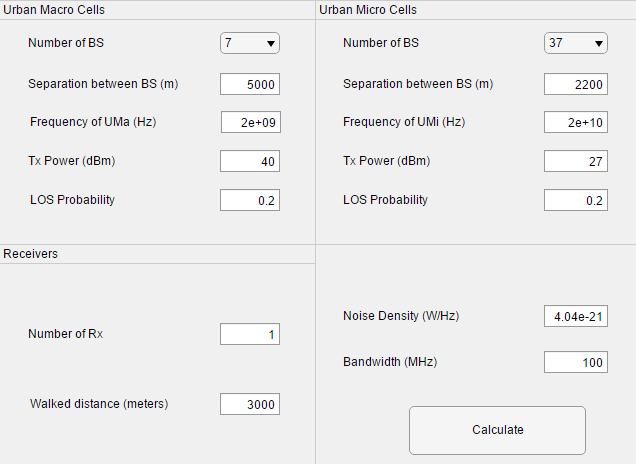
\includegraphics[width=\linewidth]{imagenes/interfaz_parametros.PNG}
	\caption{Interfaz de introducción de parámetros de simulación.}
	\label{fig:interfaz_parametros}
\end{figure}

La interfaz cuenta por defecto con unos parámetros que se han considerado estándar para una simulación 5G. El coste computacional y, por tanto, el tiempo de ejecución es directamente proporcional al número de estaciones base, de receptores y de la distancia recorrida por ellos. En el Capítulo \ref{cap.pruebas} se llevarán a cabo una serie de pruebas que mostrarán con detalle cómo varían los tiempos de ejecución en función de la exigencia del entorno simulado.

Una vez completa la simulación, se mostrará la segunda ventana gráfica donde se puede realizar las representaciones oportunas. En concreto, se pueden visualizar los valores de SINR, potencia de recepción, emparejamientos y capacidad de canal asignada a cada uno de los receptores durante su recorrido, para los casos de macro-celda y micro-celda, y para dos criterios de emparejamiento posibles: la celda de mayor SINR o la celda más cercana -Figura \ref{fig:interfaz_visualizacion}-. Además, es posible representar varios datos en la misma figura a través del \textit{checkbox} que incorpora.

\begin{figure}[h!]
	\centering
    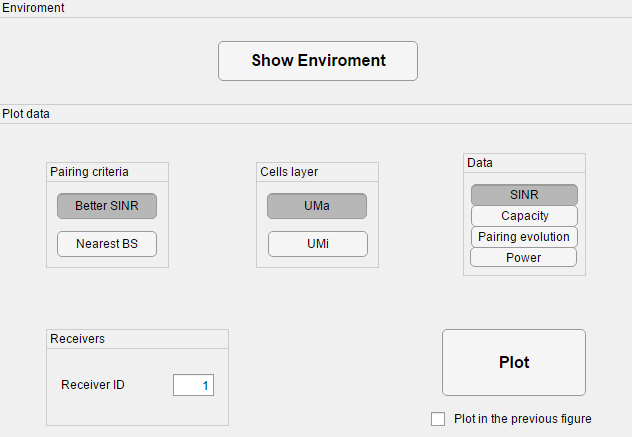
\includegraphics[width=\linewidth]{imagenes/interfaz_visualizacion.PNG}
	\caption{Interfaz de visualización de valores para las variables de salida.}
	\label{fig:interfaz_visualizacion}
\end{figure}

Una vez completa la simulación, si se atiende al \textit{workspace} de Matlab, se puede observar que se puede tener acceso a las variables de salida generadas -Figura \ref{fig:workspace}-. La naturaleza, estructura y contenido de las mismas se detallará en las secciones dedicadas a ello. Sin embargo, conviene tener en cuenta que se pueden almacenar en el disco duro a través del comando:

\begin{lstlisting}[style=Matlab-editor, basicstyle=\tiny]
save <nombre_de_fichero_de_salida>.mat
\end{lstlisting}

\begin{figure}[h!]
	\centering
    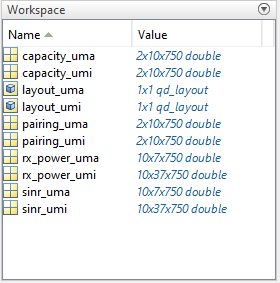
\includegraphics{imagenes/workspace.PNG}
	\caption{Workspace de Matlab tras la ejecución de una simulación.}
	\label{fig:workspace}
\end{figure}

Esto es especialmente útil cuando se quiere realizar una comparativa entre distintas simulaciones, ya que, en la actualidad, \textit{5Gneralife} solo admite la comparativa entre parámetros de salida de una misma simulación. Se estima que el fichero de salida adquiere un tamaño medio de 10 MB.

\section{Diseño}

\subsection{Planificación y concepción inicial}

Para justificar la implementación es necesario conocer previamente el planteamiento de su diseño y el proceso de concepción del mismo, puesto que una planificación debidamente estudiada es el método más eficiente para obtener un resultado de desarrollo satisfactorio.

Por ello, esta sección está dedicada a exponer las decisiones que se tomaron en la etapa de planteamiento y el motivo por el que se tomaron las mismas. De igual modo, también se justificarán los descartes de funcionalidades y simplificaciones que se adoptaron durante el proceso de implementación.

Si bien el proyecto contaba con unos objetivos flexibles desde el primer momento, como se comentaba en el Capítulo \ref{cap.requisitos}, existía una serie de requisitos para considerar el proyecto como satisfactorio una vez dada su finalización.

Estos requisitos surgen del estudio de los principales simuladores 5G existentes en la actualidad. De un rápido repaso al estado del arte del Capítulo \ref{cap.estado del arte} se puede concluir que éxito una basta gama de simuladores, pero cada uno se encuentra orientado a un propósito: desde simuladores técnicos especialmente diseñados para simulaciones que cumplan con ciertos estándares, hasta simuladores que tiene su propio modelado minimalista del comportamiento del canal y se centran en la evolución temporal de los receptores.

Sin embargo, en el momento de evaluación de alternativas no existía un simulador que reúna las principales características de todos ellos, un simulador completo que integre las normativas de simulaciones junto a evolución temporal, correlación entre cálculos y especificaciones propias de 5G como alta frecuencia o sistemas MIMO.

Es como surge \textit{5Gneralife}, el cual se concibió como una alternativa a los ya existentes, al pretender incluir evolución temporal junto a modelados de acuerdo a las diferentes normativas de simulación y la posibilidad de convivencia de celdas de distinta naturaleza en un entorno de \acs{hetnet}s.

La idea básica era basarse en la potencia que ofrece \textit{QUaDRiGa} para implementar las funciones necesarias, de modo que \textit{5Gneralife} fuera capaz de realizar un seguimiento de la señal recibida por todos los usuarios en cada instante de tiempo para todas las celdas, las cuales pueden ser de cualquier naturaleza a priori. Además, es crucial para simulaciones en 5G la incorporación de posibilidad de calcular resultados a muy altas frecuencias, puesto que la mayor novedad que incluye 5G es la de trabajar a frecuencias del orden de diez veces mayores que las que se han estado trabajando hasta ahora, así, se consiguen unas mayores tasas de transferencia y capacidades, aspecto del que se carecen estudios de comportamiento hasta la fecha.

Así, este simulador podría contribuir a realizar una mejor toma de contacto con este nuevo paradigma, junto a técnicas avanzadas como MIMO, ICIC, emparejamientos sofisticados de terminal-estación base u optimización de la planificación.

Sin embargo, por motivos de complejidad y por haberse considerado fuera del alcance de un Trabajo de Fin de Grado individual, se han descartado estas funcionalidades avanzadas y se han sustituido por simplificaciones como enlaces SISO, interfaz de conexión dual sin decisión de banda a la que conectar, emparejamientos basados en parámetros básicos y planificación geométrica con reutilización de frecuencias unitario.

Su diseño inicial se pensó como un solo \textit{script} para Matlab que integrara en él todos los cálculos y llamadas al generador de canal, cuyos resultados se pudieran estudiar a través de la línea de comandos. No obstante, al ver la relevancia de las implementaciones y de su posible mejora y escalabilidad, se decidió re-estructurar el trabajo para que fuera modular, con un arquetipo que utiliza funciones para labores específicas, y que implementa una nueva clase para reunir en un solo objeto todos los parámetros, dando así lugar a la estructura final que se presenta a continuación.

\subsection{Estructura final}

El simulador consta de un total de 14 ficheros desarrollados exclusivamente para su implementación, más todos los ficheros por los que \textit{QuaDRiGa} está constituido. 
De estos 14 ficheros, uno de ellos es el archivo principal, \textit{main.m}, que es el que se debe ejecutar para iniciar el simulador. Por otro lado, dos de los otros ficheros corresponden a las dos ventanas por las que está formada la interfaz gráfica. El resto son funciones dedicadas a realizar cálculos específicos, desde el cálculo de la SINR hasta la generación de coeficientes de canal, o bien, dedicadas a representar gráficamente los resultados.

De este modo, se puede realizar un diagrama de flujo en el que se detallan los pasos que realiza el simulador a la hora de ejecutarse, mostrando el orden de las funciones de las que se sirve en cada paso, como se especifica en la Figura \ref{fig:diagrama_simulador}:

\begin{figure}[h!]
	\centering
    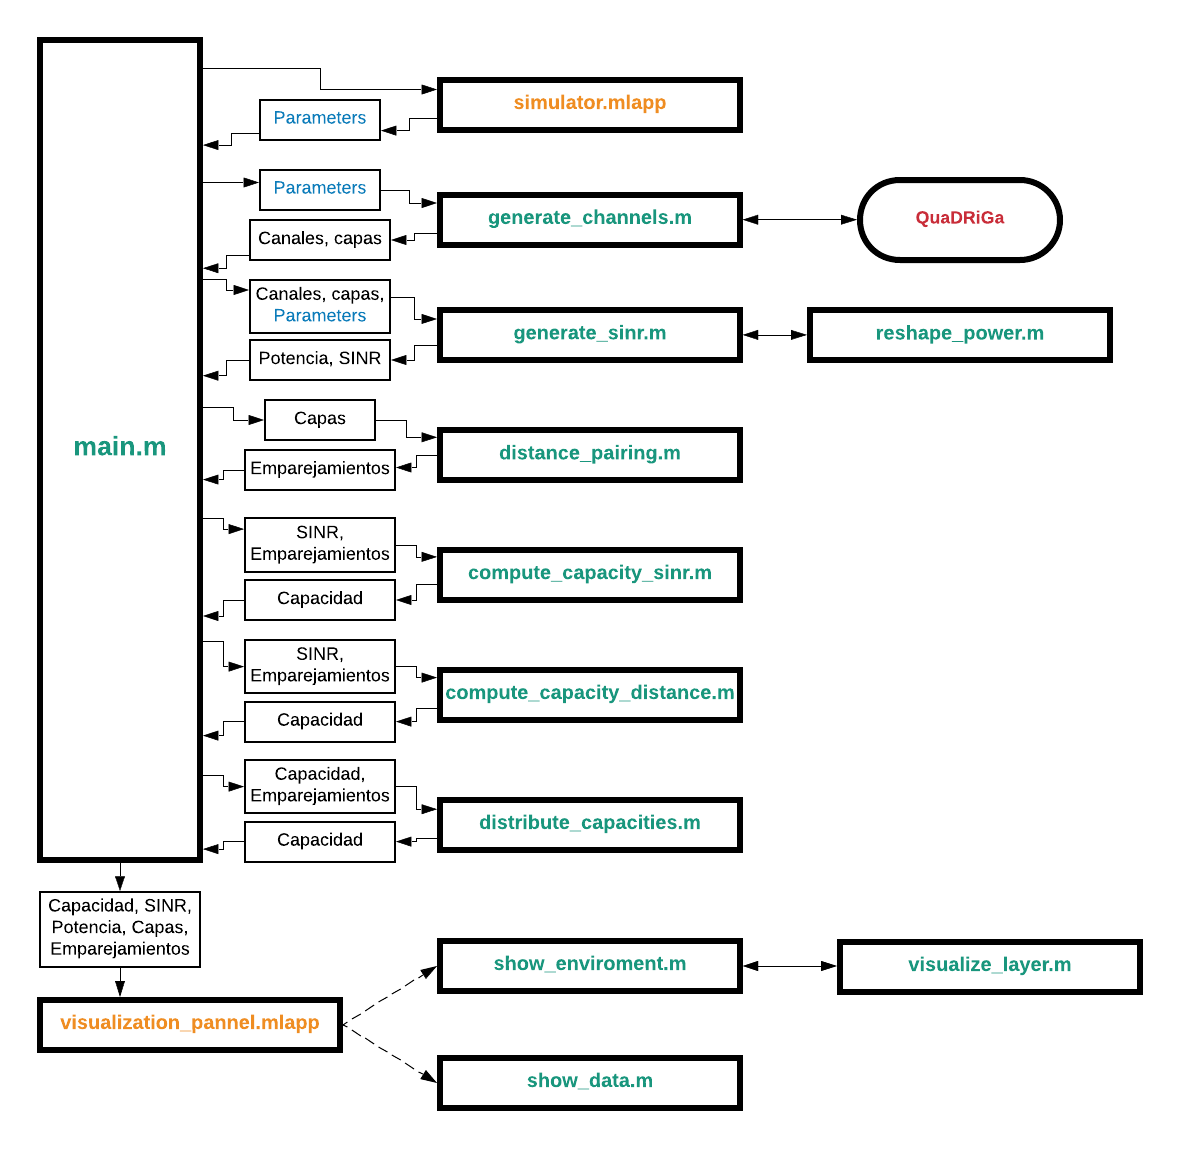
\includegraphics[width=\linewidth]{imagenes/diagrama_simulador.png}
	\caption{Diagrama de flujo del simulador.}
	\label{fig:diagrama_simulador}
\end{figure}

Además, se puede completar el anterior diagrama mostrando las etapas en las que se hace uso del cómputo de \textit{QuaDRiGa}, añadiendo las clases de las que se hace uso en cada momento -Figura \ref{fig:diagrama_simulador_completo}-:

\begin{figure}[h!]
	\centering
    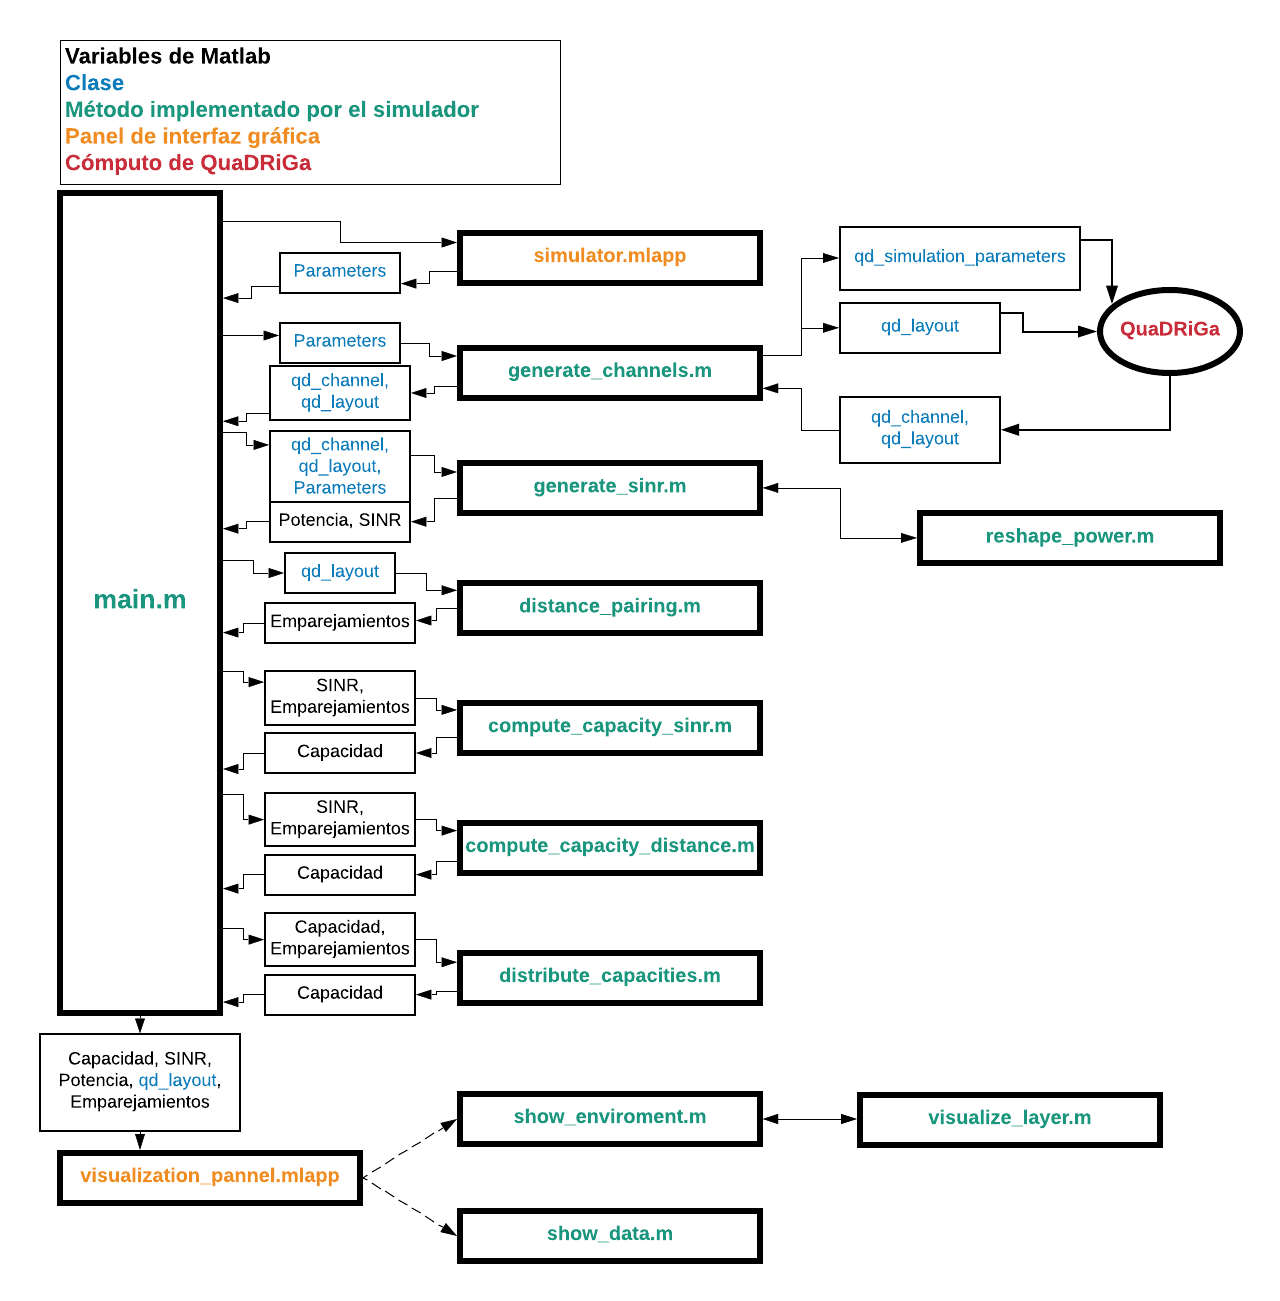
\includegraphics[width=\linewidth]{imagenes/diagrama_simulador_completo.png}
	\caption{Diagrama de flujo del simulador incluyendo las clases de \textit{QuaDRiGa}.}
	\label{fig:diagrama_simulador_completo}
\end{figure}

Como se puede observar, cada uno de los módulos en verde o en naranja, es decir, los implementados por el usuario, están dedicados a una tarea específica y son totalmente sustituibles y escalables. De este modo se facilitan las futuras implementaciones, como podría ser un tercer criterio de emparejamiento, una forma distinta de calcular la SINR o simplemente un nuevo parámetro como atributo de la clase \textit{Parameters}.

Por lo general, cada uno de los anteriormente citados módulos implementa una o varias mejoras de las listadas en la anterior sub-sección, o forman parte de una de ellas. El modo de implementación de dichas mejoras así como el código de las mismas se detallará en la siguiente sección. 

\section{Implementación}

\subsection{Implementación del diseño}

Antes de realizar el desarrollo de las funciones propias del simulador, es necesario llevar a cabo un desarrollo del diseño propuesto a partir de los elementos disponibles por parte de \textit{QuaDRiGa}. Esto implica modificar, generar y establecer una serie de parámetros que no son visibles para el usuario, puesto que en la fase de diseño se decidió que no sean modificables, con la finalidad de establecer las bases de la simulación y de este modo ajustar todas las configuraciones para que sean compatibles con 5G y el simulador posteriormente desarrollado.

En primer lugar, se ha establecido como único modelo de canal el de 3GPP TR-38.901 \cite{3gpphighfreq} el cual establece un modelado para el canal de radio de la comunicación para altas frecuencias. Aunque \textit{QuaDRiGa} ya de por sí incorpora soporte para la incorporación de este modelo de canal sin nada más que especificar que se desea utilizar el mismo, conviene conocer los detalles de lo que implica utilizar este modelado.

\begin{table}[h!]
\centering
\caption{Implicaciones de adoptar el estándar de 3GPP TR 38.901 para las implementaciones}
\label{tab:tr38901}
\begin{tabular}{|l|m{4cm}|m{4cm}|} \hline
\textbf{Característica} & \textbf{Micro-celda urbana}                                                              & \textbf{Macro-celda urbana}                                                              \\ \hline
Capa de celdas          & Hexagonal con 3 sectores por cada estación base. Distancia mínima entre celdas de 200 m. & Hexagonal con 3 sectores por cada estación base. Distancia mínima entre celdas de 500 m. \\ \hline
Visión directa          & LOS y NLOS.                                                                              & LOS y NLOS.                                                                              \\ \hline
Altura de BS            & 10 m.                                                                                    & 25 m.                                                                                    \\ \hline
Antenas                 & 3 sectores por base.                                                                     & 3 sectores por base.                                                             \\ \hline       
\end{tabular}
\end{table}

Según la Tabla \ref{tab:tr38901} de implicaciones, se establece una altura de 10 m y de 25 m para las estaciones base de micro-celdas y macro-celdas respectivamente, a la misma vez que el modelado de las antenas se hacen en tres sectores 

Por otro lado, en cuanto a la antena de transmisión, se ha utilizado la misma para ambos tipos de estación base. Se trata de una antena sectorial de aproximadamente 120º de apertura, replicada dos veces más para conseguir una cobertura total de 360º. Esta antena es compatible con todos los rangos de frecuencia por lo que es reutilizable para cualquier tipo de estación base. Se puede observar un plano de su radiación normalizada en dos dimensiones en la Figura \ref{fig:radiacion}, teniendo en cuenta que esta variará según la frecuencia y la potencia de transmisión.

\begin{figure}[h!]
	\centering
    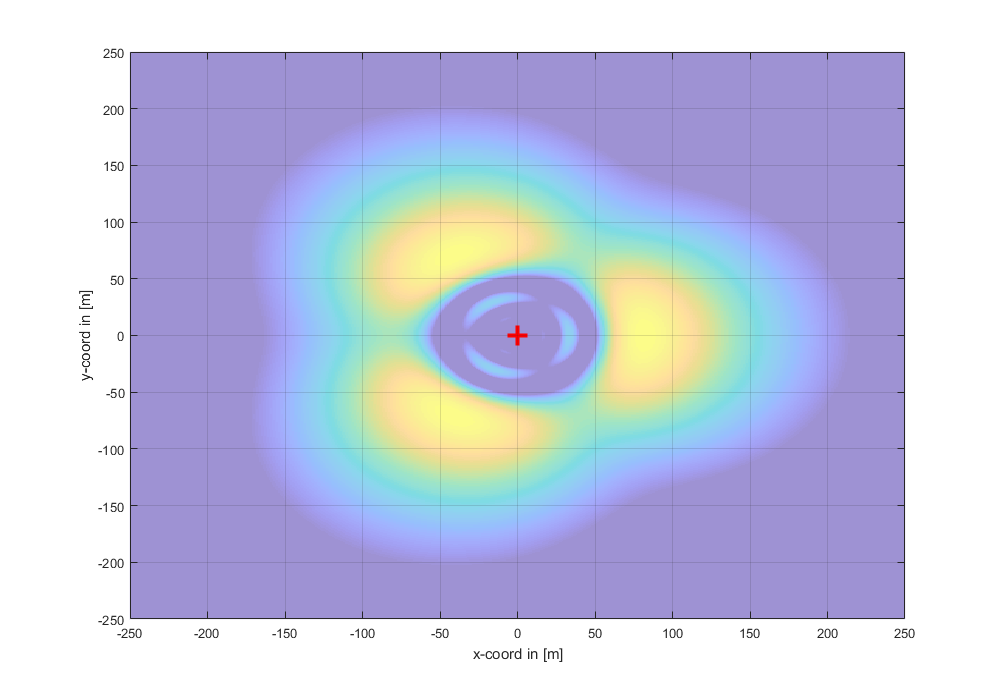
\includegraphics[width=\linewidth]{imagenes/articulo_radiacion.png}
	\caption{Esquema de radiación de la antena utilizada para los transmisores.}
	\label{fig:radiacion}
\end{figure}

Estas configuraciones para hacer posible su compatibilidad se han implementado a través del siguiente código en sus pertinentes ficheros:

\begin{lstlisting}[style=Matlab-editor, basicstyle=\tiny]
scenarios_uma = {'3GPP_38.901_UMa_LOS', '3GPP_38.901_UMa_NLOS'};
scenarios_umi = {'3GPP_38.901_UMi_LOS', '3GPP_38.901_UMi_NLOS'};

%% Antennas
aMT = qd_arrayant('omni');
aBS = qd_arrayant ('multi', 8, 0.5 , 12 );
aBS.combine_pattern;
aBS_umi = aBS.copy;

layout_uma = qd_layout.generate ('regular', params.number_of_uma, params.dist_between_uma, aBS);
layout_umi = qd_layout.generate ('regular', params.number_of_umi, params.dist_between_umi, aBS_umi);

layout_uma.tx_position(3,:) = 25; % 25 m BS height
layout_uma.set_scenario('3GPP_38.901_UMa',[],[],0,1-los_uma);

layout_umi.tx_position(3,:) = 10; % 10 m BS height
layout_umi.set_scenario('3GPP_38.901_UMi',[],[],0,1-los_umi);
\end{lstlisting}

\subsection{Implementación de mejoras}

A grandes rasgos, se puede considerar el simulador como una caja negra en la que se introducen una serie de parámetros sobre la simulación deseada y esta devuelve los valores numéricos sobre diversas características del entorno simulado. Debido a la gran cantidad de parámetros de entrada y de salida disponibles, la mejor forma de tenerlos en consideración es a través de un esquema gráfico:

\begin{figure}[h!]
	\centering
    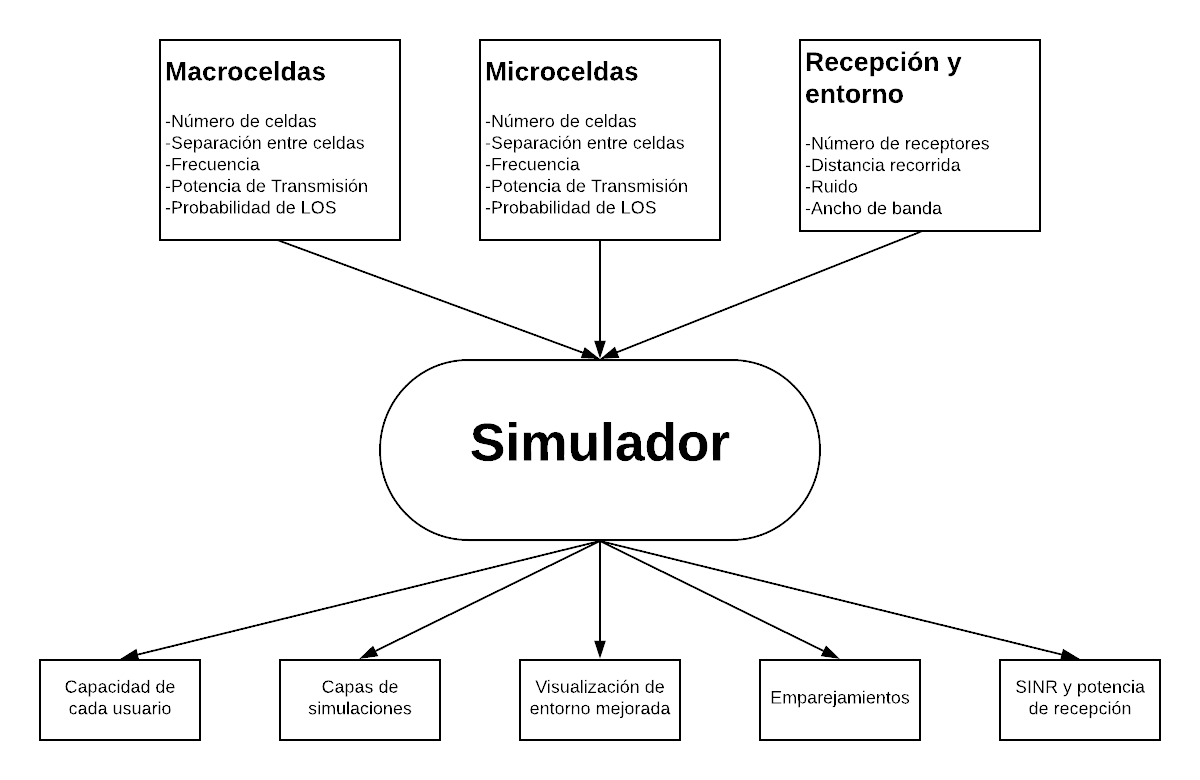
\includegraphics[width=\linewidth]{imagenes/cajanegra_simulador.png}
	\caption{Esquema de la relación de entrada y salida del simulador.}
	\label{fig:cajanegra}
\end{figure}

Estos resultados se obtienen gracias al desarrollo de las mejoras con respecto a \textit{QuaDRiGa}. Gracias a ello, el software resultante puede considerarse un simulador completo y funcional con características propias de nivel de enlace y de nivel de sistema, puesto que es capaz de evaluar emparejamientos y establecimientos de enlace a la misma vez que calcula parámetros de utilización como la capacidad o \textit{throughput}.

Centrándonos en la implementación, esta se puede resumir detallando las siete mejoras desarrolladas que se han enunciado con anterioridad, puesto que son las tareas donde se ha centrado la labor de programación, haciendo especial hincapié en ampliar las características de \textit{QuaDRiGa}. Por ello, a continuación se detalla el procedimiento de implementación de cada una de las mejoras con la finalidad de ilustrar la tarea de desarrollo y sus resultados. 

En cuanto al código, resulta importante mencionar que ha sido completamente escrito en inglés para facilitar su distribución y uso, puesto que existe una gran comunidad científica internacional que ha utilizado \textit{QuaDRiGa} para sus investigaciones y es probable que \textit{5Gneralife} les resulte atractivo. Además, así se posibilita una mayor participación en la plataforma colaborativa donde ha sido publicado el código. El mismo ha sido completamente documentado y comentado, y utiliza técnicas de programación como nombres de variables y de funciones descriptivos para facilitar su comprensión mientras se revisa y/o modifica.

\paragraph{Implementación de la Mejora 1: Recolección de datos de entrada} \mbox{} \\

Una de las problemáticas que se encontraron acerca del uso de \textit{QuaDRiGa} fue precisamente el establecimiento de parámetros de simulación. Este generador incorpora los parámetros en distintas clases de modo que es necesario especificarlos uno por uno a la misma vez que se atiende a qué clase corresponde cada parámetro.

Por ello, se ha decidido solventar este problema unificando todos los parámetros que se han considerado interesantes para su variación en una nueva clase implementada, mientras que aquellos parámetros que se ha decidido que permanezcan constantes, se han excluido de dicha clase y se han establecido a lo largo del código de todo el simulador de forma estática.

Esta implementación se ha llevado a cabo mediante la clase \textit{Parameters}, contenida en el fichero \textit{Parameters.m}. En esta versión inicial del simulador, implementa un total de 14 atributos, uno por cada parámetro de entrada, dos métodos que tienen como finalidad la de convertir la potencia de transmisión a unidades lineales y por último un constructor.

Se ha optado por establecer como públicos todos los atributos y métodos por simplificación, en lugar de implementar por cada uno de los atributos un método \textit{get} y otro método \textit{set}, que son típicos cuando se utiliza el paradigma de programación orientada a objetos. De este modo, se puede acceder y modificar directamente estos parámetros. Se puede observar la implementación de sus atributos y métodos en el siguiente código:

\begin{lstlisting}[style=Matlab-editor, basicstyle=\tiny]
    properties
        freq_uma; % UMa Frequency in Hz
        freq_umi; % UMi Frequency in Hz
        number_of_uma; % Number of Macro-cells
        number_of_umi; % Number of Micro-cells
        dist_between_uma; % Distance between UMa cells center
        dist_between_umi; % Distance between UMi cells center
        number_of_rx; % Number of Mobile Terminals
        walked_distance; % Distance that Mobile Terminals will walk in meters
        tx_power_uma; % Transmit Power of UMa BS in dBm
        tx_power_umi; % Transmit Power of UMi BS in dBm 
        BW; % Asigned bandwidth to each BS in MHz
        No; % Noise in W/Hz
        los_uma; % LOS probability for UMa enviroment
        los_umi; % LOS probability for UMi enviroment
    end
    
    methods
        function pow = get_lin_pow_uma(obj)
            pow = 10^(obj.tx_power_uma/10); % Power in W
        end
        function pow = get_lin_pow_umi(obj)
            pow = 10^(obj.tx_power_umi/10); % Power in W
        end
    end
\end{lstlisting}

\paragraph{Implementación de la Mejora 2: Combinación de capas de simulación independientes} \mbox{} \\

El mayor impedimento con el que cuenta \textit{QuaDRiGa} a la hora de simular entornos heterogéneos es la independencia entre sus capas de simulación y la imposibilidad de combinarlas. Recuérdese que el entorno de simulación se encuentra implícito en el objeto de los receptores y no en los de las estaciones base, puesto que no existe un objeto dedicado a ellas. De nada sirve simular una capa de macro-celdas con usuarios aleatorios si se necesita simular una segunda capa de micro-celdas que cuenta con otros usuarios distintos aleatorios.

Por ello, se ha utilizado una versión modificada del ejemplo que se mostraba en el Capítulo \ref{cap.quadriga} para generar las dos capas de simulación y sus respectivos coeficientes de canal. Esta función funciona del mismo modo que el ejemplo anterior, con la salvedad de que se repite una segunda vez para la capa de micro-celdas. Una vez que ambas capas son creadas, se procede a crear uno a uno el objeto \textit{qd\_track} que modela el movimiento de los receptores por las calles de Berlín a lo largo de la distancia especificada por el usuario del simulador. Lo que hace especial esta parte es que este objeto, antes de serle asignado un entorno de simulación, es copiado a ambas capas de simulación. De este modo, ambas capas tendrán un usuario idéntico, con el mismo recorrido, pero con distintos segmentos, distintos puntos de transición de LOS a NLOS y viceversa, y distintos tipos de celda asignados:

\begin{lstlisting}[style=Matlab-editor, basicstyle=\tiny]
prob_uma = [los_uma, 1-los_uma];
prob_umi = [los_umi, 1-los_umi];

scenarios_uma = {'3GPP_38.901_UMa_LOS', '3GPP_38.901_UMa_NLOS'};
scenarios_umi = {'3GPP_38.901_UMi_LOS', '3GPP_38.901_UMi_NLOS'};

%% Write all streets in one layout

for a = 1 : params.number_of_rx
    trk = qd_track('street', params.walked_distance, randi(360), 50, 87, 83, 10, 0.85); % Street
    trk.initial_position = layout_uma.rx_position(:,a); % Strat-pos
    trk.name = layout_uma.rx_name{a};  % Unique name
    layout_uma.track(1,a) = trk{1}.copy; % Assign to layout
    layout_uma.track(1,a).set_scenario( scenarios_uma, prob_uma, 10 ,30, 12 );
    layout_umi.track(1,a) = trk{1}.copy;
    layout_umi.track(1,a).set_scenario( scenarios_umi, prob_umi, 10 ,30, 12 ); % Segments
end
\end{lstlisting}

\paragraph{Implementación de la Mejora 3: Modelado de potencia de transmisión y de SINR} \mbox{} \\

La única salida que ofrece \textit{QuaDRiGa} es la de un objeto que entre su contenido se encuentran los coeficientes de canal del enlace -clase \textit{qd\_channel}-.  Estos coeficientes pretenden modelar las comunicaciones del canal de modo que cada comunicación individual entre un transmisor y un receptor tenga un coeficiente característico que contenga la relación entre la señal emitida y la recibida.

En la Figura \ref{fig:esquema_comunicacion} se puede apreciar el esquema de una situación típica en la que un transmisor, $Tx_1$, se comunica con \textit{M} receptores. En total habrá una cantidad de \textit{M} enlaces establecidos, uno por cada receptor, en los que la amplitud de la señal se verá afectada así como su fase una vez recibida.

\begin{figure}[h!]
	\centering
    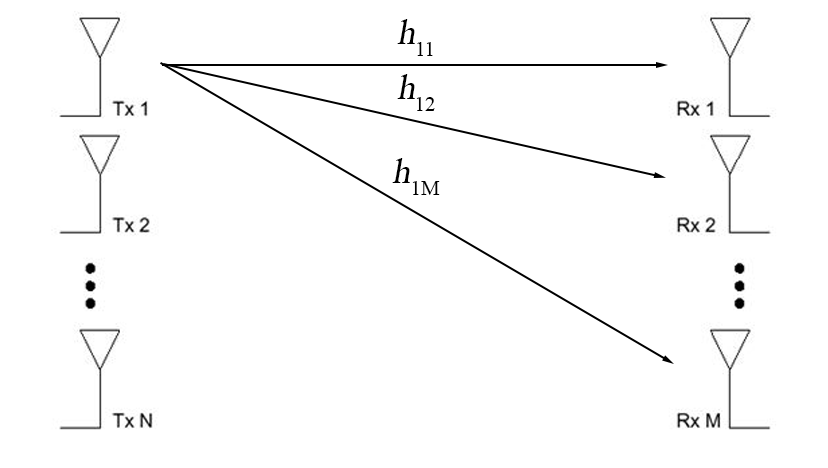
\includegraphics[width=0.85\linewidth]{imagenes/esquema_comunicacion.png}
	\caption{Esquema de comunicación en un entorno con varios receptores y emisores.}
	\label{fig:esquema_comunicacion}
\end{figure}

Por tanto, se puede considerar el canal como una función de transferencia $H$ que modifica la amplitud y la fase de la señal \cite{modelado}. Es decir, se trata de una función de transferencia compuesta por una matriz de dimensiones \textit{NxM}, siendo \textit{N} el número de transmisores y \textit{M} el número de receptores, cuyos coeficientes son números complejos con un módulo que resulta en la relación entre amplitudes, y con una fase que incorpora el desfase entre señales -Figura \ref{fig:matrizcanal}-.

\begin{figure}[h!]
	\centering
    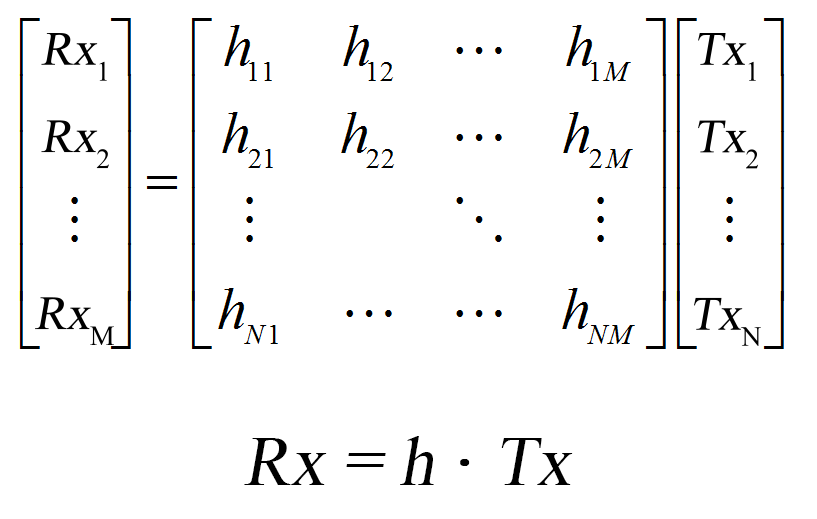
\includegraphics[width=0.75\linewidth]{imagenes/matriz_canal.png}
	\caption{Matriz del canal y relación entre coeficientes.}
	\label{fig:matrizcanal}
\end{figure}


Donde $h_ij$ es un coeficiente complejo que contiene la información de la relación entre la señal transmitida por el transmisor $Tx_i$ y la señal recibida por el receptor $Rx_j$ \cite{matrizcanal}. \textit{QuaDRiGa} almacena estos coeficientes en la matriz de cuatro dimensiones que se describía en el Capítulo \ref{cap.quadriga}. Dicha matriz se almacena en el atributo \textit{coeff} de la clase \textit{qd\_channel}.

Aunque el desfase puede resultar en interferencias destructivas debido al modelo de rayo de 20 trayectorias, cuya superposición pueda resultar en una interferencia consigo misma, para la estimación de la potencia se ha despreciado este posible efecto y solamente se ha atendido al módulo de los coeficientes.

Ya que \textit{QuaDRiGa} no implementa la posibilidad de inclusión de potencia de transmisión, se ha realizado una implementación sencilla de cálculo de potencia de recepción a través del módulo de la matriz de canal. En concreto, teniendo en cuenta que se trabaja con unidades lineales, la potencia de recepción se encuentra definida por:

$$ P_{Rx_i} = |h_{ij}|^2 * P_{Tx_j} (W) $$

Para \textit{5Gneralife} se ha implementado esta funcionalidad a partir de la introducción de la potencia de transmisión en dBm y convirtiendo dicho valor a unidades lineales -vatios- a través del método dedicado a ello de la clase \textit{Parameters}. El cálculo de potencias se realiza para cada uno de los enlaces, esto quiere decir que se necesita un total de interacciones igual al producto del número de receptores, el número de transmisores total y el número de muestras tomadas -por defecto, una muestra por cada metros recorrido-. Estos cálculos han sido implementados en la función \textit{generate\_sinr} que está dedicada precisamente al cálculo de potencia de recepción y a la SINR a través de la debida extracción de los coeficientes de canal:

\begin{lstlisting}[style=Matlab-editor, basicstyle=\tiny]
for a = 1 : number_of_rx
    power = zeros( layout.no_tx*3 , no_snap_per_track );
    for builder = 1 : layout.no_tx
        power_calc = abs(channel(a,builder).coeff).^2;
        power_calc = sum( power_calc, no_sectors_per_bs );
        power_calc = reshape( power_calc, no_sectors_per_bs, no_snap_per_track );         % 3 sectors per BS

        index = (builder-1)*no_sectors_per_bs+1 : builder*no_sectors_per_bs;
        power(index,:) = power_calc * tx_power;
    end

    rx_aux(a, :, :) = power;
end
\end{lstlisting}

Esto realiza un cálculo de la potencia para cada receptor en cada instante de tiempo. Sin embargo, la característica más interesante a la hora del estudio de una red de comunicaciones inalámbricas no es la potencia de recepción, sino la relación de esta frente al ruido y al resto de señales del entorno, también conocida como SINR. Por ello, gracias a la integración de ruido térmico como parámetro de entrada, se puede modelar este parámetro a partir de la recopilación de todas las potencias de transmisión \cite{capacity}:

\[SINR_i = \frac{P_{BS_i}}{N_{o} - P_{BS}(i) + \sum_{j = 1}^{N} P_{BS_j}}\]

Siendo $P_{BS_i}$ la potencia recibida por la estación base \textit{i}, $N_o$ el ruido térmico en W y $N$ el número de estaciones base a la misma frecuencia que la estación base \textit{i}.

Esta implementación se ha realizado mediante el cálculo iterativo de la SINR para todos los receptores considerando todos los posibles casos de enlace, con la finalidad de determinar en cada instante de tiempo la SINR de todas las estaciones base y así poder compararlas entre sí, lo cual facilita la tarea de elección de la mejor SINR para emparejamientos:

\begin{lstlisting}[style=Matlab-editor, basicstyle=\tiny]
for i = 1:number_of_rx
    aux = rx_aux(i,:,:);
    aux = reshape(aux, [layout.no_tx*3, no_snap_per_track]);
    current_rx_pow = reshape_power(aux);

    for j = 1:layout.no_tx
        for k = 1:no_snap_per_track
            sinr(i,j,k) = current_rx_pow(j,k) / ...
                (sum(current_rx_pow(:, k)) + No - current_rx_pow(j,k));
        end
    end

    sinr(i,:,:) = 10*log10(sinr(i,:,:));
    rx_power(i, :, :) = current_rx_pow;
end
\end{lstlisting}

\paragraph{Implementación de la Mejora 4: Criterios de emparejamiento} \mbox{} \\

Existe en la actualidad una gran diversidad de métodos de emparejamiento de terminales móviles que determinan la mejor estación base dependiendo de múltiples criterios. Este factor puede resultar decisivo en la eficiencia de la red y en posibles congestiones, puesto que determina con qué intensidad se está utilizando la infraestructura, sin dejar de tener en cuenta que los recursos de la red siempre son limitados.

Aunque la variedad de algoritmos de emparejamiento puede dar pie a un estudio mucho más exhaustivo, lo suficiente como para surgir otro proyecto independiente, para la implementación del simulador se ha decidido que, por limitación de tiempo y para priorizar otros aspectos del desarrollo, solamente se han tenido en cuenta dos criterios como se venía comentando anteriormente: emparejamiento con la estación base más cercana y emparejamiento con la estación base de mayor SINR recibida.

Para su implementación, simplemente se explora la matriz de SINR o la matriz de distancias, dependiendo del caso, con la finalidad de almacenar en una matriz de emparejamientos el índice de la estación base correspondiente. Esta selección se realiza a través de la función \textit{distance\_pairing} para el emparejamiento por distancia y mediante un sencillo recorrido del máximo de la variable SINR en el fichero principal de ejecución.

Emparejamiento por SINR:

\begin{lstlisting}[style=Matlab-editor, basicstyle=\tiny]
for j = 1:no_snap
    for i = 1:params.number_of_rx
        [~, pairing_uma(1,i,j)] = max( sinr_uma(i,:,j) );
        [~, pairing_umi(1,i,j)] = max( sinr_umi(i,:,j) );
    end
end
\end{lstlisting}

Emparejamiento por distancia:

\begin{lstlisting}[style=Matlab-editor, basicstyle=\tiny]
for i = 1:snap
    for j = 1:no_rx
        for k = 1:no_tx
            pos_rx = layout.track(j).positions(:,i) + layout.track(j).initial_position(:);
            pos_tx = layout.tx_position(:,k);
            distances(j,i,k) = sqrt(sum((pos_rx-pos_tx).^2));
        end
    end
end
    
for i = 1:snap
    for j = 1:no_rx
        [~, indice] = min(distances(j,i,:));
        pairing(j,i) = indice;
    end
end
\end{lstlisting}

\paragraph{Implementación de la Mejora 5: Cálculo capacidad de canal} \mbox{} \\

Uno de los factores en los que más énfasis se hace para futuras implementaciones de 5G es el de asignación de ancho de banda. Debido a las grandes tasas de transferencia que se espera y a la gran cantidad de usuarios, es primordial un reparto del ancho de banda disponible eficiente.

Para \textit{5Gneralife} se ha diseñado una mecánica de reparto de ancho de banda que se rige por la compartición equitativa por parte de todos los usuarios conectados a una misma celda o estación base, a la cual se ha pre-asignado un ancho de banda predeterminado de acuerdo con el parámetro especificado por el usuario del simulador.

Este ancho de banda asignado se encuentra directamente relacionado con una característica que afecta directamente a la experiencia del usuario: la tasa de transferencia máxima, también conocida como capacidad de canal o \textit{troughput}. Esta tasa de transferencia es un factor clave en usos de la red orientadas a multimedia, como vídeo o descargas, puesto que determinará el tiempo que tardará un fichero en descargarse o la calidad máxima que un \textit{streaming} de vídeo podrá adoptar para una calidad de servicio satisfactoria.

Para este simulador, se ha implementado la siguiente ecuación que se sirve de la SINR y del ancho de banda asignado a cierto usuario para determinar su máxima tasa de transferencia \cite{capacity}:

$$C = BW · \log_{2}( 1 + SINR(dB) ) (MBit/s) $$

Puesto que la SINR obtenida dependerá de la estación base o celda a la que se ha vinculado el receptor en cuestión, el cálculo dependerá estrechamente del criterio de emparejamiento. Por tanto, para un mismo receptor y una misma capa de simulación en un mismo instante de tiempo, se obtendrán dos valores de \textit{throughput} diferentes: uno para el caso de emparejamiento con la celda más cercana y otro para el caso de emparejamiento con la celda de mayor SINR.

Aunque resulta intuitivo que, puesto que la SINR está directamente relacionada con el resultado calculado de capacidad, la mayor capacidad se dará en el caso de conexión a la estación base de mejor SINR, existen casos en los que esta suposición no es correcta, puesto que el ancho de banda varía en función del número de terminales móviles conectados a la estación base estudiada. Por tanto, los resultados variarán sustancialmente dependiendo de si en el caso simulado existe congestión en una o más celdas.

La implementación de esta característica se ha llevado a cabo mediante las funciones \textit{compute\_capacity\_sinr} y \textit{compute\_capacity\_sinr}, dedicadas a calcular la capacidad en el caso de emparejamiento de la mejor SINR o de la menor distancia, respectivamente. Para ello, toman como parámetros de entrada la SINR anteriormente calculada, o bien, los objetos de capas para calcular la distancia hasta el centro de las celdas, dependiendo del caso, así como la matriz de emparejamientos.

Código de implementación para el caso de mejor SINR -\textit{compute\_capacity\_sinr}-:
\begin{lstlisting}[style=Matlab-editor, basicstyle=\tiny]
for i = 1:dimension(1)
    for j = 1:dimension(3)
        sinr_dist(i,j) = sinr(i, pairing(1, i, j), j);
    end
end
sinr_dist(sinr_dist < 0) = 0;
capacity(:,:) = BW*log2(1+sinr_dist);
\end{lstlisting}

Código de implementación para el caso de celda más cercana -\textit{compute\_capacity\_distance}-:
\begin{lstlisting}[style=Matlab-editor, basicstyle=\tiny]
for i = 1:dimension(1)
    for j = 1:dimension(3)
        sinr_dist(i,j) = sinr(i, pairing(2, i, j), j);
    end
end
sinr_dist(sinr_dist < 0) = 0;
capacity(:,:) = BW*log2(1+sinr_dist);
\end{lstlisting}

\paragraph{Implementación de la Mejora 6: Visualización mejorada} \mbox{} \\

Aunque esta no es una funcionalidad fundamental de los simuladores de comunicaciones, ya que estos suelen estar orientados a los estudios cuantitativos y la extracción de datos de los entornos generados, en numerosos casos resultan útiles las representaciones gráficas de las simulaciones en cuanto a disposición de elementos se refiere.

Sin embargo, al tratarse de un generador y modelador de canal generalista, las funciones que \textit{QuaDRiGa} relacionadas con la representación visual pueden resultar un poco escuetas e incompletas, sobre todo en casos con escenarios sobrecargados de usuarios, donde puede ser difícil visualizar dónde se encuentra el receptor en cuestión.

Por ello, aunque no sea una característica propia de un simulador técnico, se ha decidido emplear una porción del tiempo disponible para el proyecto en mejorar la visualización nativa de \textit{QuaDRiGa} e incorporar funciones como la de representar varias capas al mismo tiempo -antes solo se podían representar las capas individualmente ya que el método de representación estaba implementado en la clase \textit{qd\_layout}-, distinguir fronteras entre celdas -implementado gracias a la función de Matlab \textit{voronoi}- o representar la trayectoria de los receptores de una forma más estética, asignando también un color diferente a cada uno de ellos.

Esta mejora se ha implementado mediante una función dedicada exclusivamente a representar las dos capas de simulación en una misma figura, junto a la separación entre ellas distinguida según el color -rojo para macro-celdas y verde para micro-celdas-, y el seguimiento de la trayectoria de los usuarios. Aunque se ha necesitado modificar parte del código del método original de \textit{QuaDRiGa} para moldear algunos aspectos de la visualización, se ha decidido implementar una modificación del método en el mismo directorio \textit{src} del simulador con la finalidad de sobre-escribir el original sin realizar ninguna modificación en el código de \textit{QuaDRiGa} descargado.

La función \textit{show\_enviroment} muestra dicha representación avanzada sin necesidad de llamar a ninguna otra función o método, mientras que la versión modificada de \textit{qd\_layout.visualize} se ha implementado en una función llamada \textit{visualize\_layer}:

\begin{lstlisting}[style=Matlab-editor, basicstyle=\tiny]
figure('position', [50 50 900 600]) % Adjust figure position

color = ['g', 'r']; % Colors of layouts
    
parameter = [2, 1];
    
for i = 1:2
    pos = l(i).tx_position';
    hold on
    visualize_layer(l(i),[],[], parameter(i), 0, i); % visualize layout
    hold on
    handel_prop = voronoi(pos(:,1),pos(:,2),'k'); % Division between cells
    set(handel_prop(1),'Color',color(i)); % Split lines
    aux=size(handel_prop,1);
    for j=2:aux
        set(handel_prop(j),'LineWidth',3, 'Color', color(i)); % Adjust colors
    end
    hold on
end
    
h = zeros(3, 1);
h(1) = plot(NaN,NaN,'^r'); % Legend elements
h(2) = plot(NaN,NaN,'^g');
h(3) = plot(NaN,NaN,'ob');
legend(h, 'UMa BS position','UMi BS position','Rx position');
    
view(-33,48)
hold off
\end{lstlisting}

Por otro lado, también resulta atractiva la visualización gráfica de los datos de salida obtenidos, en este caso, SINR, capacidad de canal, potencia de recepción y evolución de emparejamientos. Por ello, se ha implementado una segunda función dedicada a plasmar estos datos en la totalidad del recorrido por parte del receptor en una figura, incluyendo en la figura una leyenda generada automáticamente así como descripción de los ejes.

% Figura representando

La implementación se ha llevado a cabo teniendo en cuenta toda la casuística posible, facilitando la entrada de datos a la misma con la intención de que pueda ser fácilmente integrada para ser llamada desde otras funciones automáticamente, sin necesidad de un uso manual de la misma, aunque esto es también posible -leer documentación HTML del código, descrita en la siguiente sub-sección-.

\begin{lstlisting}[style=Matlab-editor, basicstyle=\tiny]
len = length( input(1,1,:) );
dist = 1:len;

switch data
    case 'SINR'
        index_data = 1;
    case 'Power'
        index_data = 2;
    case 'Pairing'
        index_data = 3;
    case 'Capacity'
        index_data = 4;
end

if strcmp(criteria, 'SINR')
    crit = 1;
else
    crit = 2;
end

%% Ploting
%data_for_plotting = zeros(1:len);
title_gen = ['of the Rx' num2str(rx_id,'%02d')];

if hold_on == 0
    figure;
else
    hold all
end

display_name = ['Repr. of ' data ' ' title_gen ' at ' type...
    ' layer paired by ' criteria];

switch index_data
    case 1
        for i = 1:len
            paired = pairing(crit, rx_id, i);
            data_for_plotting(i) = input(rx_id, paired, i);
        end
        plot( dist, data_for_plotting, 'DisplayName', display_name )
        title(['SINR ' title_gen ' in the ' type ' layer'])
        ylabel('SINR [dB]')
    case 2
        for i = 1:len
            paired = pairing(crit, rx_id, i);
            data_for_plotting(i) = input(rx_id, paired, i);
        end
        data_for_plotting = 10*log10(data_for_plotting);

        plot( dist, data_for_plotting, 'DisplayName', display_name )
        title(['Received Power ' title_gen ' in the ' type ' layer'])
        ylabel('Power [dBm]')
    case 3
        for i = 1:len
            data_for_plotting(i) = pairing(crit, rx_id, i);
        end
        plot( dist, data_for_plotting, 'DisplayName', display_name )
        title(['Pairing evolution ' title_gen ' in the ' type ' layer'])
        ylabel('Number of the associated BS')
        maximum = max(data_for_plotting);
        ylim([0.9 maximum(1)+0.3])
    case 4
        for i = 1:len
            data_for_plotting(i) = input(crit, rx_id, i);
        end
        plot( dist, data_for_plotting, 'DisplayName', display_name )
        title(['Capacity ' title_gen ' in the ' type ' layer'])
        ylabel('Capacity [MBit / second]')
end
xlim([0,len])
xlabel('Walked distance [m]')
legend('-DynamicLegend');

if hold_on
    hold off
end
\end{lstlisting}

\paragraph{Implementación de la Mejora 7: Interfaz gráfica de usuario} \mbox{} \\

Gran parte de la problemática de uso de \textit{QuaDRiGa} reside en la curva de aprendizaje de dicho software, ya que su nivel de abstracción hace que a veces resulte abrumador para un usuario novel. Por ello, buscando una solución que facilite el modo de uso del simulador, se determinó que la mejor manera de llevar a cabo esta tarea es la de implementar una interfaz gráfica de usuario que permita usar el simulador en apenas unos cuantos clics.

Para este tipo de desarrollo, Matlab facilita su labor incorporando ciertas herramientas que permiten diseñar aplicaciones y/o ventanas gráficas sin necesidad de diseñarlas desde cero. Es el caso de la tradicional \textit{GUIDE} y de la recientemente incorporada \textit{App Designer}, las cuales se conciben para facilitar la creación de ventanas de aplicación de una forma gráfica sin estricta necesidad de escribir código para ello. Por la gran cantidad de herramientas, flexibilidad y facilidad de uso, se decidió utilizar \textit{App Designer} en lugar de \textit{GUIDE} aun teniendo en cuenta que al tratarse de una incorporación de la versión 2017a de Matlab, su compatibilidad iba a verse reducida con respecto al caso de haber utilizado \textit{GUIDE}.

\begin{figure}[h!]
	\centering
    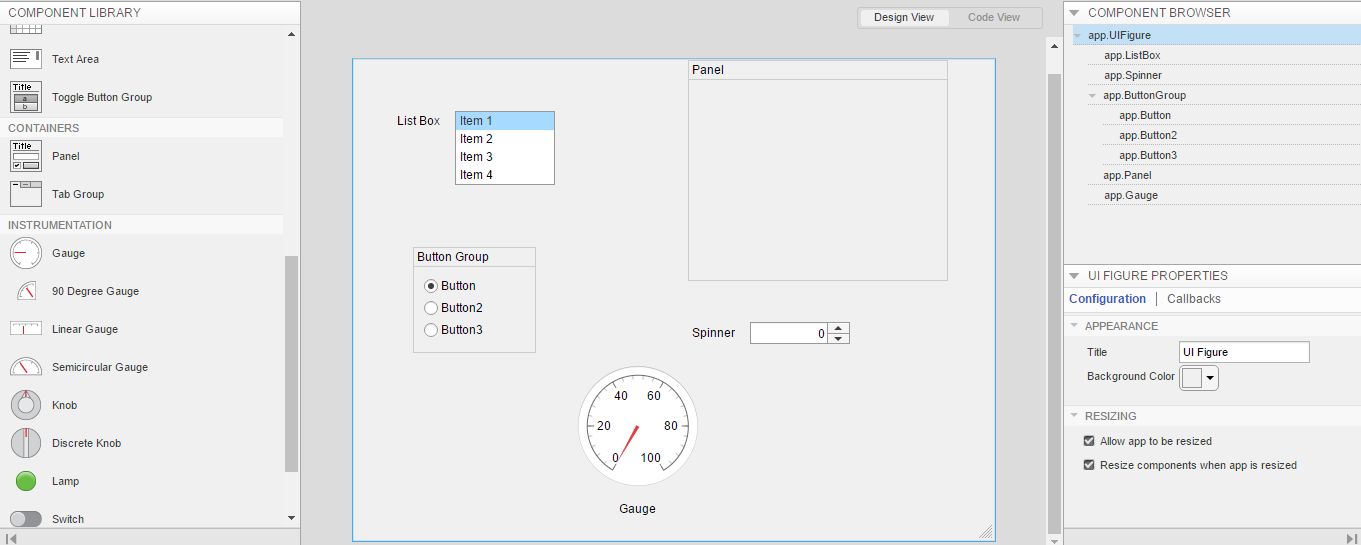
\includegraphics[width=\linewidth]{imagenes/interfaz_appdesigner.PNG}
	\caption{Interfaz de \textit{App Designer}.}
	\label{fig:appdesigner}
\end{figure}

\textit{App Designer} tiene una forma simple de uso: colocar los elementos requeridos en la ventana creada, arrastrándose intuitivamente con el puntero del ordenador. Estos elementos, por lo general, sirven para introducir datos o realizar una acción, como es el caso de los botones. Una vez incorporados todos los elementos deseados, se configura uno o varios botones con la finalidad de que al ser pulsados se realice una acción determinada por el código interno de la figura. En este caso, se diseñaron dos tipos de ventana: una de introducción de datos cuyo único botón procede a la ejecución de la simulación con los datos introducidos, y otra para determinar qué datos de salida se desea que sean representados gráficamente, a través de botones mayormente.

\begin{figure}[h!]
	\centering
    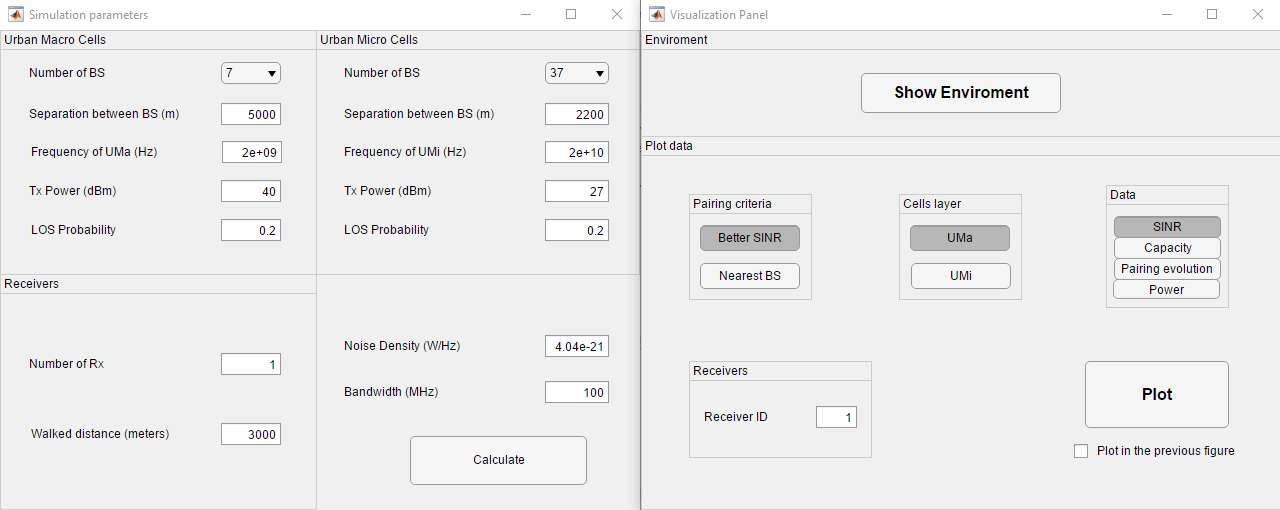
\includegraphics[width=\linewidth]{imagenes/ventanas.PNG}
	\caption{Interfaces gráficas de usuario que constituyen \textit{5Gneralife}.}
	\label{fig:ventanas_graficas}
\end{figure}

La ventana de introducción de datos cuenta con un campo de texto y/o numérico por cada uno de los atributos con los que cuenta la clase \textit{Parameters}. Su función es la de recoger cada uno de ellos y generar un objeto de dicha clase que reúna todos los parámetros deseados. A grandes rasgos, se podría decir que esta ventana implementa una interfaz gráfica del constructor de la clase \textit{Parameters}. Al pulsar el botón dedicado a cerrar la ventana y crear el objeto, se realiza una llamada a dos funciones: al constructor de \textit{Parameters} y a la función que la misma ventana incluye para cerrarse:

\begin{lstlisting}[style=Matlab-editor, basicstyle=\tiny]
            params = Parameters(app.freq_uma.Value, app.freq_umi.Value, str2double( app.number_of_uma.Value ), str2double( app.number_of_umi.Value ),...
                app.dist_between_uma.Value, app.dist_between_umi.Value, app.number_of_rx.Value, app.walked_distance.Value, app.tx_power_uma.Value, ...
                app.tx_power_umi.Value, app.BW.Value, app.No.Value, app.los_uma.Value, app.los_umi.Value);
            
            save('parameters.mat', 'params');
                
            delete(app);
\end{lstlisting}

El intercambio de variables entre el \textit{script} principal de ejecución y el código interno de la ventana se realiza a través del disco duro. La ventana almacena en el directorio principal las variables en forma de fichero para que posteriormente el \textit{script} las recoja y elimine del disco duro.

Por otro lado, en cuanto a la ventana dedicada a representar gráficamente los resultados de salida, cuenta con una constitución distinta ya que se ha concebido para facilitar las representaciones gráficas de las que dispone \textit{5Gneralife}. Esto incluye la disposición geográfica de los elementos -botón \textit{show\_enviroment}- y la representación de los valores de las variables de salida a lo largo de todo el recorrido del usuario seleccionado en \textit{Receiver ID} -SINR, capacidad, potencia, etc.-.

Para ello, al pulsar el botón \textit{Plot} se llama a la función encargada de trazar los datos en una nueva figura, pasando como argumentos las variables necesarias de acuerdo a la selección de los botones de la interfaz por parte del usuario. Esto se ha implementado a través de un \textit{script} incluido en el código interno de la ventana que evalúa el estado de cada uno de los botones seleccionables y realiza la llamada a la función de acuerdo a las opciones seleccionadas por el usuario:

\begin{lstlisting}[style=Matlab-editor, basicstyle=\tiny]
rx_id = app.no_rx.Value;
hold_on = app.holdon.Value;

if (app.uma.Value)
    type = 'UMa';
    pairing = app.pairing_uma;
else
    type = 'UMi';
    pairing = app.pairing_umi;
end

if (app.better_sinr.Value)
    criteria = 'SINR';
else
    criteria = 'Nearest BS';
end

if (app.sinr.Value)
    data = 'SINR';
    if strcmp(type,'UMa')
        input = app.sinr_uma;
    else
        input = app.sinr_umi;
    end
elseif (app.capacity.Value)
    data = 'Capacity';
    if strcmp(type, 'UMa')
        input = app.capacity_uma;
    else
        input = app.capacity_umi;
    end
elseif (app.power.Value)
    data = 'Power';
    if strcmp(type,'UMa')
        input = app.rx_power_uma;
    else
        input = app.rx_power_umi;
    end
else
    data = 'Pairing';
    input = pairing;
end

show_data(criteria, type, data, rx_id, pairing, hold_on, input);
\end{lstlisting}

\section{Documentación y publicación del código}

Puesto que \textit{QuaDRiGa} se encuentra publicado bajo Licencia Pública General Reducida de GNU, conocida por su nombre en inglés GNU \ac{lgpl} con propósitos educativos, se ha decidido seguir con la misma filosofía de publicación y el código del simulador ha sido publicado su propio repositorio en GitHub \cite{publicacion}, con el propósito de ofrecer el uso del simulador a todo aquél que lo desee, o bien, ofrecer la posibilidad de mejorar gracias a las contribuciones que cualquier colaborador puede aportar.

En dicho repositorio se encuentra la documentación HTML de todo el proyecto, con sus especificaciones sobre formas de uso, descripción de variables, comentarios de uso y ejecución, instrucciones... En él también se puede encontrar el código fuente de la presente memoria, escrita en el sistema de escritura de documentos LATEX.

De este modo, se facilita la distribución del código y se abre posibilidad a que el proyecto quede al servicio de la comunidad científica y técnica, dando lugar siempre a que el proyecto crezca.

%
\chapter{Pruebas}\label{cap.pruebas}
\section{Introducción}
Bla bla bla
%
\chapter{Conclusiones y trabajos futuros}\label{cap.conclusiones}
\section{Introducción}

En este último capítulo se va a tratar el grado de consecución de los objetivos con los que el proyecto contaba en un principio y las conclusiones que se pueden extraer a raíz de él. 

Durante el trascurso del proyecto, se ha desarrollado un simulador de redes 5G funcional a partir del generado de canal \textit{QuaDRiGa}, implementado en Matlab. Se ha conseguido que este simulador sea intuitivo a la hora de ser usado gracias a su interfaz gráfica, y como resultados, ofrece unos entornos de 5G realistas y configurables. Gracias a las herramientas implementadas, se pueden obtener representaciones gráficas del entorno y de las variables de salida, tales como SINR, \textit{throughput} o potencia recibida, atendiendo a dos criterios de emparejamiento distintos y a dos tipos de celda: macro-celda y micro-celda urbanas.

El desarrollo de este simulador ha sido llevado a cabo a través de programación modular y orientada a objetos, escrita completamente en inglés, lo que facilita la escalabilidad y comprensión por parte de un tercero. Puesto que la herramienta ha sido concebida para su uso académico, se ha publicado bajo una licencia GNU LGPL v3.0 y se ha creado un repositorio para la misma.

El simulador, aun teniendo sus limitaciones, ha demostrado ajustarse a los estándares descritos por entidades como 3GPP, integrando su compatibilidad con el TR 38.901, un modelado de canal y de entorno para 5G en los que se engloban los escenarios de alta potencia y utilización. Por tanto, el simulador implementa los recursos necesarios como para generar escenarios a frecuencias de hasta 100 GHz, con movilidad de usuarios y evolución temporal implementadas.

Sin embargo, existen características típicas de 5G que no han sido implementadas, como enlaces MIMO, modelado de celdas de naturaleza más pequeña, como pico-celdas o femto-celdas, o técnicas avanzadas como ICIC o criterios de emparejamiento más avanzados, como asignar prioridades a determinados tipos de celda.

Aun tratándose de un prototipo que adopta algunas simplificaciones para facilitar su desarrollo, integra funcionalidades de modelado de canal como parámetros de gran escala y de pequeña escala que realizan unos cálculos del modelo del canal muy exactos, tanto que dependiendo de la envergadura de la simulación, su tiempo de ejecución puede durar días.

En definitiva, el simulador \textit{5Gneralife} ha demostrado cumplir su función, proporcionando unas simulaciones que permiten evaluar el comportamiento de un escenario 5G de una forma fácil, a pesar de sus limitaciones y simplificaciones de implemetación, sirviendo como base para un posible proyecto mucho más ambicioso que podría deparar en un simulador completamente funcional y exhaustivo.

\section{Mejoras y futuros pasos}
Con el ánimo de que el proyecto se mantenga vivo y pueda seguir mejorándose, se ha publicado en su totalidad con la filosofía de software libre en la plataforma colaborativa GitHub, donde cualquier colaborador puede aportar sus implementaciones o descargarse el simulador para sus propias pruebas.

Como simulador que integra funcionalidades de nivel de enlace y de sistema, se da pie a que a través de implementaciones que lo complementen, pueda llegar a ser un proyecto que consiga evolucionar y convertirse en un simulador completo.

Como posibles tareas de mejora, se propone la implementación de un procesamiento multi-núcleo que permita acortar tiempos de ejecución. Otra característica interesante sería la del modelado de visión directa dependiendo de la distancia a la que se encuentre la estación base en cuestión. Por otro lado, una funcionalidad que resultaría en un avance considerable sería la inclusión de criterios de emparejamiento adicionales, puesto que permitiría evaluar la red desde unos criterios más realistas. También se puede hacer mención a ciertos detalles que parametrizan la red con más detalle, como puede ser la adición de pico-celdas o femto-celdas, la implementación de reuso de frecuencias para evitar interferencias, o la posibilidad de que un receptor se mueva a una velocidad determinada. 

El propio departamento de radio-comunicaciones del Fraunhofer HHI ha mostrado su interés en el proyecto, puesto que está basado en \textit{QuaDRiGa}, su propio proyecto, y actualmente se encuentra evaluando el código del simulador para la propuesta de futuras mejoras y colaboraciones.
%
%\chapter{Conclusiones y Trabajos Futuros}
%
%
%%\nocite{*}
%\addbibresource{bibliografia/bibliografia.bib}
\bibliography{./bibliografia/bibliografia}
\bibliographystyle{unsrt}
%
%\appendix
%\input{apendices/manual_usuario/manual_usuario}
%%\input{apendices/paper/paper}
%\input{glosario/entradas_glosario}
% \addcontentsline{toc}{chapter}{Glosario}
% \printglossary
\chapter*{}
\thispagestyle{empty}

\end{document}
